\documentclass[11pt]{article}
\usepackage[T1]{fontenc}
\usepackage[utf8]{inputenc}
\usepackage{lmodern}
\usepackage[margin=1in]{geometry}
\usepackage{amsmath,amssymb,amsthm,mathtools}
\usepackage{graphicx}
\usepackage{booktabs}
\usepackage{array}
\usepackage{tabularx}
\usepackage{xcolor}
\usepackage[numbers,sort&compress]{natbib}
\usepackage{microtype}
\usepackage{longtable}
\usepackage[section]{placeins}
\usepackage[colorlinks=true,linkcolor=blue!50!black,citecolor=blue!50!black,urlcolor=blue!50!black]{hyperref}

\newtheorem{theorem}{Theorem}
\newtheorem{proposition}[theorem]{Proposition}
\newtheorem{lemma}[theorem]{Lemma}
\newtheorem{corollary}[theorem]{Corollary}
\theoremstyle{definition}
\newtheorem{definition}[theorem]{Definition}
\newtheorem{remark}[theorem]{Remark}
\newtheorem{finding}[theorem]{Finding}

\newcommand{\tr}{\operatorname{tr}}
\newcommand{\E}{\mathbb{E}}
\newcommand{\R}{\mathbb{R}}
\newcommand{\PSD}{\mathbb{S}_{+}}
\newcommand{\gap}{\mathrm{gap}}
\newcommand{\tbd}[1]{\textcolor{red}{[#1]}}
\newcolumntype{L}{>{\raggedright\arraybackslash}X}
\graphicspath{{figures/}}
\newcommand{\TT}{ZIT-25}% the 25-step, CFG 4, pooled Z-Image Turbo campaign (archive files labelled Z-Image Base)

\title{Projection, Pooling and Tangent Agreement:\\
Equivalence Relations for Layerwise Spectral Trajectories\\ of Generative Transformers\\[4pt]
\large Mode-II: the mathematical companion}
\author{Zac Doyle\\ \small mode:LIMINAL\\ \small ORCID \href{https://orcid.org/0009-0006-0452-1374}{0009-0006-0452-1374}\\ \small \url{https://github.com/Z-L-D/mode-II}}
\date{November 2026\\ \small Version of 11 November 2026}

\begin{document}
\maketitle

\begin{abstract}
This is a measurement-theoretic companion to an empirical atlas of layerwise spectral telemetry (Mode-I), which records a normalised participation ratio $g$, the leading singular-value gap and the spectral entropy $H$ of the token activation matrix at every layer and sampling step of generative transformers. It states what these coordinates can and cannot see and which nulls an observation in them must beat. The pieces are elementary lemmas, a taxonomy and a checklist; it is a theory of the instrument's limits, not of the models.

Three results carry the paper. First, pooling the two branches of classifier-free guidance can only raise $g$ above the energy-weighted branch mean (a trace concavity), so the capture functional is a confound of known sign for $g$; the theorem says nothing about the gap or $H$. Assuming approximately equal branch energies, which the archive did not log and which a later capture (Mode-I Round 18) finds close in most cells (median conditional-to-unconditional trace ratio $1.004$--$1.021$), its size on identical trajectories is $+0.040$ to $+0.088$ in $\log g$: enough to reverse a scalar-envelope ordering, too small to produce the tangent tiers. Second, an invariance classification: the triple sees only part of the normalised spectrum, and set against the networks' own symmetries the telemetry is blind to every rotation of an RMSNorm residual stream but, under adaptive normalisation, as in every image and audio transformer of the atlas, only to signed channel permutations; depth-tangent agreement is necessary, not sufficient, for an orthogonal correspondence. In the archive $\log g$ and $H$ are nearly monotone in each other, so the triple is effectively two-dimensional. Third, eight conditions that a strong, trajectory-level and capture-independent universality claim in these coordinates must meet; weaker claims need only those that apply to the statistic they name. As exact relations, shape and tangent agreement of standardised profiles coincide; they differ as graded statistics, and the tangent's power lies in how it weights depth frequencies.

Claim boundary: no result in the archive meets all eight conditions. We also bound envelope correlations below by shared trends, derive differencing and surrogate nulls and sample-size-robust onset estimators, and show, against a same-weights null, that a residual depth field does not transfer between depth-matched unrelated models. The theory explains none of Mode-I's effect sizes.
\end{abstract}

\begin{center}
\fbox{\begin{minipage}{0.94\linewidth}\small
\textbf{Main results and notation.}
\begin{itemize}\setlength\itemsep{1pt}
 \item \emph{Pooling theorem} (Thm.~\ref{thm:pool}): pooled CFG capture raises $g$ above the energy-weighted branch mean; the capture functional is a confound of known sign.
 \item \emph{Trend dominance} (Prop.~\ref{prop:trend}): scalar envelope correlations are bounded below by shared trends and cannot identify a vector field.
 \item \emph{Invariance} (Lemma~\ref{lem:rot}): what the triple cannot see; a high tangent is necessary, not sufficient, for an orthogonal correspondence.
 \item \emph{Taxonomy of comparison levels} (Def.~\ref{def:levels}): envelope, field, shape and tangent. As exact relations, field equality implies shape and envelope equality, and shape and tangent equality coincide on standardised profiles; as graded statistics the four differ, and the tangent's value lies in how it weights depth frequencies. A taxonomy, not a theorem about the data. The tangent is calibrated only between depth-matched models (\S\ref{sec:tangent}); the empirical tiers are in Mode-I \S5.3--5.4.
 \item \emph{Flow family}: $\partial_uz=F_m(z,u,\tau)$, model-specific and non-autonomous; no shared microscopic $F$ for the pairs tested (an empirical finding, Finding~\ref{fd:nofield}).
 \item \emph{Nulls and estimators} (Prop.~\ref{prop:diff}, \S\ref{sec:nulls}, \S\ref{sec:estimators}): the differencing null, two surrogate classes and the relative onset.
 \item \emph{Claim boundary} (\S\ref{sec:universality}): eight conditions for a strong universality claim in these coordinates. Table~\ref{tab:kinds} lists which results are proved, assumed or measured.
\end{itemize}
Notation: $z=(g,\gap,H)$; $u\in[0,1]$ normalised depth; $\tau$ the sampling state, identified with the noise level $\sigma$ for flow-matching and diffusion models (so $\tau$ and $\sigma$ name the same axis; $u$ is depth, never time); $m$ model, $p$ prompt, $s$ seed; $\beta_\ell=g(\ell+1)-g(\ell)$ the layer step, $b(g)=\E[\beta\mid g]$ the analyzer's binned flow; $\rho_{\rm tan}$ the tangent statistic (Def.~\ref{def:levels}). Campaign labels: ZIT (Z-Image Turbo, 8 steps), \TT{} (Turbo, 25 steps, archive files labelled Z-Image Base), Z1/Z2/Z3 (real Base CFG 4, Base CFG 1, Turbo at Base settings), ACEB/ACET (ACE-Step Base/turbo). R$n$-$k$ and S$k$: preregistered predictions; D$k$: cards of the project's internal findings ledger (available on request); RC$k$: post hoc review checks. CoS-PAFS: the Chain-of-Steps Phase-Adaptive Flow Solver project, whose capture node and analyzer are used. Same weights: two captures of one checkpoint; lineage pair: two related checkpoints, either \emph{distillation lineage} (a Base model and its distilled student) or \emph{successor lineage} (a later model of one vendor and line whose training relation is not documented, SD3$\to$SD3.5 Medium), or \emph{sibling lineage} (two models derived separately within one family, Z-Image Base and Turbo). Native grid: a depth grid with one point per hooked layer of the shallower model of a pair. The comparison statistics' nulls and sizes come from Mode-I; Appendix~\ref{app:imports} lists every imported result with its evidence class. In \S\ref{sec:linear} the gap enters with a minus sign, $z=(g,-\gap,H)$. Gates G1--G4 (standing requirements for claims not made here): response under perturbation, an independent distillation pair with quality labels, cloned continuations for commitment, context-invariant language-model statistics.
\end{minipage}}
\end{center}


\begin{table}[htbp]
\centering\footnotesize
\caption{What each result is: proved, assumed or measured. Theorems hold whatever the data; their use on the archive depends on the assumptions in the third column; findings are measurements imported from or shared with Mode-I and can be overturned by new captures.}
\label{tab:kinds}
\begin{tabularx}{\linewidth}{@{}>{\raggedright\arraybackslash}p{3.4cm}>{\raggedright\arraybackslash}p{1.9cm}L@{}}
\toprule
Result & Kind & Assumptions or evidence\\
\midrule
Pooling bound, Thm.~\ref{thm:pool} & theorem & none beyond PSD branch moments; controls $g$ only\\
Equal-energy forms, Thm.~\ref{thm:pool} (last line), Cor.~\ref{cor:eq} & theorem & equal branch energies; on the data an assumption, close in most cells where logged (Round 18)\\
Measured pooling increments ($+0.040$ to $+0.088$) & finding & conditional on near-equal branch energies, not logged for the archive\\
Trend dominance, Prop.~\ref{prop:trend} & theorem & the fitted-slope sign condition stated there\\
Invariance of the triple, Lemma~\ref{lem:rot} & theorem & none; (iv) by explicit certificate\\
Symmetry classes, Cor.~\ref{cor:rot} & theorem & (c) needs channel-separating modulations, an assumption about trained weights not measured in the archive\\
Exact relations of Def.~\ref{def:levels} & elementary facts & every coordinate varies across depth\\
Differencing null, Prop.~\ref{prop:diff} & theorem & Gaussian, or independent sub-Gaussian coordinates after whitening; effective rank growing\\
Fitted fields do not transfer, Finding~\ref{fd:nofield} & finding & the model class \eqref{eq:flow}, these coordinates and the pairs tested\\
Tangent tiers and the related--unrelated split & finding (Mode-I) & depth-matched pairs; five unrelated model pairs; ordering within related pairs a hypothesis\\
Eight universality conditions, \S\ref{sec:universality} & requirements & for a strong, trajectory-level, capture-independent claim\\
\bottomrule
\end{tabularx}
\end{table}

\tableofcontents
\newpage

%=====================================================================
\section{Problem statement}\label{sec:problem}

\paragraph{Objects.} A generative model $m$ is run on a prompt $p$ with seed $s$. Diffusion and flow models are sampled on a decreasing noise schedule $\sigma_0=1>\sigma_1>\dots>\sigma_{T-1}$; we write $\tau\in[0,1]$ for the sampling clock and use $\sigma$ itself as the coordinate whenever two models share a schedule. At sampling state $\tau$ and transformer block $\ell\in\{1,\dots,L_m\}$, a forward hook records the token activation matrix $X_{m,p,s}(\ell,\tau)\in\R^{N\times D}$ of one submodule (attention or MLP output). We use normalised depth $u=(\ell-1)/(L_m-1)\in[0,1]$ so that models of different depth can be compared.

\paragraph{Observed state.} The archive stores only three spectral statistics of each $X$, collected in
\begin{equation}
 z_{m,p,s}(u,\tau)=\big(g,\ \gap,\ H\big)\in(0,1]\times[1,\infty)\times[0,\log D],
\end{equation}
defined in \S\ref{sec:observables}. The full hidden state is never observed. All results below are therefore about trajectories of $z$, a low-dimensional projection of a very high-dimensional dynamical system, and every equivalence we define is an equivalence of projected trajectories.

\paragraph{Five kinds of similarity.} For two models $a$ and $b$ we distinguish:
\begin{enumerate}
 \item \emph{trajectory (envelope) similarity}: agreement of a scalar summary such as the layer-mean $\bar g(\tau)$;
 \item \emph{field similarity}: agreement of the population field $(u,\tau)\mapsto \E_{p,s} z(u,\tau)$;
 \item \emph{shape similarity}: agreement of depth profiles after per-state standardisation;
 \item \emph{content-relational similarity}: agreement of the prompt-by-prompt distance structure;
 \item \emph{tangent (dynamical) similarity}: agreement of the depth derivative $\partial_u z$ at matched sampling state.
\end{enumerate}
The main structural fact of the archive is that these five relations rank model pairs differently (\S\ref{sec:hierarchy}, \S\ref{sec:content}). Throughout, \emph{same weights} means one checkpoint under changed inference (steps, guidance, capture branch), and \emph{lineage} means two related checkpoints: a distilled checkpoint and its undistilled source (distillation lineage), a later model of one vendor and line (successor lineage), or two models derived separately within one family, neither from the other (sibling lineage: Z-Image Base and Turbo, whose teacher is an unreleased SFT model).

\paragraph{What is not claimed.} We do not claim full-state conjugacy or orbit equivalence between models, a renormalisation-group universality class, thermodynamic criticality, a separatrix or commitment boundary in the sampling dynamics, or any link between this geometry and output quality. Section~\ref{sec:universality} states what a stronger claim would require.

\paragraph{Provenance.} All quantities are computed by scripts released with the companion paper and this one; every empirical number cites the round of the audit trail in which it was obtained and whether it was preregistered. Where the archive mixes capture regimes, the regime is named (\S\ref{sec:capture}).

%=====================================================================
\section{Spectral observables}\label{sec:observables}

\subsection{The uncentred second moment}
Let $X\in\R^{N\times D}$ and $M=X^\top X/N\in\PSD^D$, the uncentred second-moment matrix. Its eigenvalues are $\lambda_1\ge\dots\ge\lambda_D\ge 0$ and we write $s_i=\sqrt{\lambda_i}$, the singular values of $X/\sqrt N$. No mean is subtracted: the token mean, which in transformer activations is often dominated by a few large channels \citep{sun2024massive}, is part of the measured geometry. In joint text--image sequences the hooked rows also include the caption tokens: in Z-Image the 64 caption rows carry at least $98\%$ of the uncentred MLP energy in every layer from 10 to 26 (layer means over 8--29: $0.96$ Turbo, $0.99$ Base), and $40$--$100\%$ in deep attention (Round 11; Mode-I \S5.3), so there the statistic describes caption tokens more than image tokens. Section~\ref{sec:open} returns to what this implies.

\subsection{Definitions}
\begin{definition}[Spectral state]
\begin{align}
 g(X) &= \frac{1}{D}\,\frac{\big(\sum_i s_i\big)^2}{\sum_i s_i^2}
 = \frac{\|X\|_*^2}{D\,\|X\|_F^2} = \frac{(\tr\sqrt{M})^2}{D\,\tr M},\label{eq:g}\\
 \gap(X) &= s_1/s_2,\qquad
 H(X) = -\sum_i q_i\log q_i,\quad q_i = s_i\Big/\sum_j s_j .
\end{align}
\end{definition}
Here $\|\cdot\|_*$ is the nuclear norm and $\|\cdot\|_F$ the Frobenius norm. By Cauchy--Schwarz, $\|X\|_*^2\le \operatorname{rank}(X)\,\|X\|_F^2$, so $g\in[1/D,\ \operatorname{rank}(X)/D]$, with $g=1/D$ exactly for rank one and $g=1$ for a flat spectrum of full rank. We call $D g$ the \emph{amplitude participation ratio}: $g$ measures how flat the singular-value spectrum is, from $1/D$ for a single direction to $1$ for a fully isotropic matrix.

\begin{remark}[Relation to other dimension measures]\label{rem:dims}
Three related quantities should not be confused. The eigenvalue participation ratio $(\sum\lambda_i)^2/\sum\lambda_i^2$ \citep{gao2017theory,recanatesi2022scaledependent} uses $\lambda_i=s_i^2$ and weights the top of the spectrum more heavily. The effective rank of \citet{roy2007effective} is $\exp(H)$, the exponential of the entropy we record separately, with $H=-\sum_i\tilde p_i\log\tilde p_i$ and $\tilde p_i=s_i/\sum_js_j$: singular values, not their squares, are normalised (natural logarithm throughout). Our $g$ is the amplitude version: it is the squared ratio of the nuclear to the Frobenius norm, divided by $D$. All three are Schur-concave functions of the normalised spectrum and agree on the extremes, but they are not monotone transformations of each other. All three are also dimensions of a covariance-type matrix, so they depend on the choice of variables (Lemma~\ref{lem:rot} makes this exact for the triple), unlike dimensions derived from a Lyapunov spectrum, which are invariant under smooth changes of coordinates; in a random recurrent network the two kinds move differently as the coupling grows, the participation ratio rising monotonically while the attractor dimension saturates and then falls \citep{clark2026lyapunov}. In the archive itself, $\log g$ and $H$ are close to monotone in each other (Spearman $0.93$--$0.97$ over all cells of the eight passive cubes, depth profiles correlated at $0.92$--$0.98$), while $\log\gap$ is only partly determined by either ($-0.79$ to $-0.20$); the triple is effectively two-dimensional, with the gap as the second coordinate (Round 10, descriptive; per-cube values for all 20 cubes of the record, where the range widens to $0.85$--$0.98$ and $-0.79$ to $+0.09$, are in Supplement Table~\ref{tab:collin}, post hoc RC31). The two-dimensionality does work in the tier analysis: the tangent weights its three coordinates equally, so $\log g$ and $H$ together count twice, and the one lineage cell that fails on a single coordinate (ACE-Step MLP on the gap alone, Mode-I Table~8) is in the model where the gap is least tied to the other two (Spearman $+0.09$ with $\log g$ in turbo MLP). Every comparison level built on the triple therefore lives close to a two-dimensional coordinate system, which bounds how much any statistic on it can discriminate between models; the tiers survive on $\log g$ or $H$ alone (Mode-I RC18), which is what near-collinearity of those two predicts.
\end{remark}

\subsection{Capture functionals}\label{sec:capture}
With classifier-free guidance \citep{ho2022classifierfree}, each sampling step evaluates the network on a conditional branch $X_c$ and an unconditional branch $X_u$. A hook can record different functionals of the pair:
\begin{itemize}
 \item \emph{pooled}: the statistic of the stacked matrix $\binom{X_c}{X_u}$, whose second moment is $M_{\mathrm{pool}}=\tfrac12(M_c+M_u)$;
 \item \emph{conditional only}: the statistic of $X_c$;
 \item \emph{branch mean}: the average of the two branch statistics.
\end{itemize}
These are different functionals of the same forward pass. The archive contains all three, sometimes within one campaign (Mode-I, \S3.2). The next section shows that the choice alone moves $g$ by a predictable sign.

\begin{figure}[t]
 \centering
 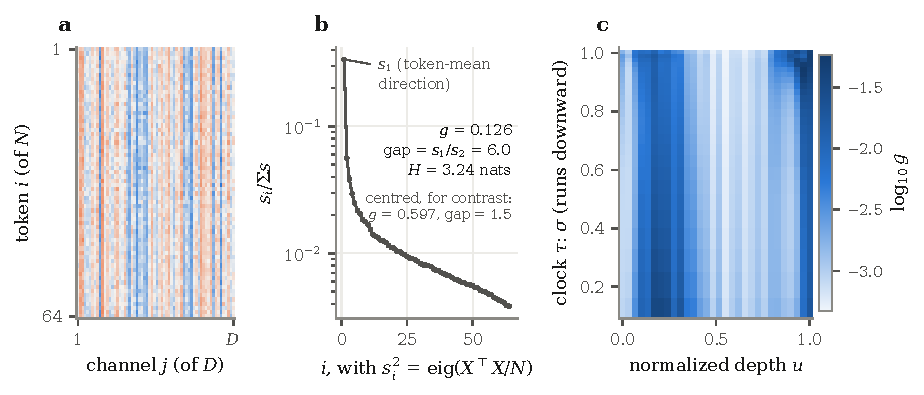
\includegraphics[width=\linewidth]{II-F1_observable_stack}
 \caption{\textbf{Mathematical observable stack.} (a) Illustration: a simulated token matrix $X\in\mathbb{R}^{N\times D}$ with a non-zero token mean. The instrument keeps the mean, so it uses the uncentred second moment $C=X^\top X/N$. (b) Illustration: the amplitude spectrum $s_i=\sqrt{\lambda_i(C)}$ of the same matrix, with $g$, gap and $H$ computed from it. The leading amplitude $s_1$ follows the token-mean direction. Centring the same matrix gives a very different $g$ and gap, so $g$ and gap partly measure the ratio of mean to fluctuation. (c) The observed field $\log_{10} g(u,\sigma)$ for Z-Image Turbo MLP at 25 steps (\TT{}, archive files labelled Z-Image Base; archive, pooled CFG 4 capture, 476 generations, mean over generations). It is plotted on normalized depth $u=L/(L_{\max}-1)$ and the sampling clock $\tau=\sigma$. Panels (a) and (b) are illustrations; (c) is measured data from the raw telemetry cube.}
 \label{fig:stack}
\end{figure}

%=====================================================================
\section{A pooling theorem}\label{sec:pooling}

\begin{lemma}\label{lem:phi}
The map $\Phi:\PSD^D\to\R_{\ge0}$, $\Phi(M)=(\tr\sqrt M)^2$, is concave and positively homogeneous of degree one.
\end{lemma}
\begin{proof}
Homogeneity is immediate: $\Phi(cM)=(\sqrt c\,\tr\sqrt M)^2=c\,\Phi(M)$. Concavity is the case $p=1/2$ of the concavity of $A\mapsto(\tr A^p)^{1/p}$ on $\PSD^D$ for $0<p\le1$, proved by \citet{carlen2008minkowski} in the more general form $(\tr\sum_jA_j^p)^{1/p}$. For completeness, an elementary route: the square root is operator concave on $\PSD^D$ \citep{bhatia1997matrix,ando1979concavity}, hence $M\mapsto\tr\sqrt M$ is concave \citep{carlen2010trace}. The superlevel set $\{\Phi\ge1\}=\{\tr\sqrt M\ge1\}$ is therefore convex, and by homogeneity every superlevel set $\{\Phi\ge c\}=c\{\Phi\ge1\}$ is convex, so $\Phi$ is quasi-concave. A nonnegative, quasi-concave function that is positively homogeneous of degree one is concave (a standard fact, proved directly here; see \citealp[\S3.4]{boyd2004convex}): for $A,B$ with $\Phi(A),\Phi(B)>0$, put $\hat A=A/\Phi(A)$, $\hat B=B/\Phi(B)$, so $\Phi(\hat A)=\Phi(\hat B)=1$; with $\theta=\Phi(A)/(\Phi(A)+\Phi(B))$, quasi-concavity gives $\Phi(\theta\hat A+(1-\theta)\hat B)\ge1$, i.e.\ $\Phi(A+B)\ge\Phi(A)+\Phi(B)$, and superadditivity plus homogeneity is concavity ($\Phi(\theta A+(1-\theta)B)\ge\Phi(\theta A)+\Phi((1-\theta)B)=\theta\Phi(A)+(1-\theta)\Phi(B)$). The case $\Phi(A)=0$ (i.e.\ $A=0$) is trivial.
\end{proof}

\begin{theorem}[Pooling raises $g$ above the energy-weighted branch mean]\label{thm:pool}
Let $X_1,\dots,X_K$ be branch activation matrices with $N_k$ rows each, let $\pi_k=N_k/\sum_jN_j$, and let $X_{\mathrm{pool}}$ be their row concatenation. Write $E_k=\tr M_k=\|X_k\|_F^2/N_k$ for the branch energies and $g_k=g(X_k)$. Then
\begin{equation}\label{eq:pool}
 g(X_{\mathrm{pool}})\ \ge\ \sum_{k}\omega_k\,g_k,\qquad \omega_k=\frac{\pi_kE_k}{\sum_j\pi_jE_j},
\end{equation}
with equality if the $M_k$ are proportional to one another. For commuting $M_k$ (a common eigenbasis) proportionality is also necessary for equality: $\Phi$ is then $\|\lambda\|_{1/2}$ of the eigenvalue vector, and equality in the reverse Minkowski inequality for $p=1/2$ holds only for proportional vectors. For non-commuting $M_k$ the equality cases are open; the use made of the theorem (a confound of known sign) does not need them. In particular, with equal branch energies, $g_{\mathrm{pool}}\ge\frac1K\sum_k g_k$ when $\pi_k=1/K$.
\end{theorem}
The theorem controls $g$ only, not the gap or $H$, and is an inequality: how loose it is in practice is measured, not proved (median slack $0.43$ in $\log$ over random branch pairs; `How tight the bound is' below).
\begin{proof}
$M_{\mathrm{pool}}=\sum_k\pi_kM_k$ and $\tr M_{\mathrm{pool}}=\sum_k\pi_kE_k$. By \eqref{eq:g}, $D\,g(X)\,\tr M=\Phi(M)$. Lemma~\ref{lem:phi} gives $\Phi(M_{\mathrm{pool}})\ge\sum_k\pi_k\Phi(M_k)=D\sum_k\pi_kE_kg_k$; divide by $D\tr M_{\mathrm{pool}}$. If $M_k=c_kM$ for all $k$, both sides equal $g(M)$ because $g$ is scale invariant.
\end{proof}

\begin{corollary}[What was tested]\label{cor:eq}
With equal energies, $\sqrt{g_{\mathrm{pool}}}\ge\tfrac1K\sum_k\sqrt{g_k}$. This follows from Theorem~\ref{thm:pool} and Jensen's inequality, or directly from the concavity of $\tr\sqrt\cdot$.
\end{corollary}

\begin{remark}[Energy weights matter]\label{rem:energy}
Without equal energies the unweighted bound $g_{\mathrm{pool}}\ge\frac1K\sum g_k$ can fail: a high-$g$ branch with small energy contributes little to the pooled spectrum. Two draw schemes give two rates. Scheme A (\texttt{pooling\_bound\_check.py}: 2{,}000 pairs, $D=8$, 30 rows per branch, Gaussian rows with Gamma(0.5) channel scales, each branch scaled by a uniform factor in $[0.2,5]$): the unweighted inequality fails in 275 pairs ($13.8\%$). Scheme B (Fig.~\ref{fig:pool}a: 20{,}000 pairs, $D=2$--$32$, random rank, a shared mean component, a log-normal energy factor with $\sigma=1$): the unweighted inequality $g_{\rm pool}\ge\frac1K\sum g_k$ fails in 1{,}000 pairs ($5.0\%$) and the weaker square-root form of Corollary~\ref{cor:eq} in 841 ($4.2\%$). Every rate quoted in this paper is one of these three. The rate depends on how the pairs are drawn, and only its being non-zero matters; while \eqref{eq:pool} held in 5{,}000 of 5{,}000 draws with minimum slack $1.2\times10^{-11}$ (script \texttt{pooling\_bound\_check.py}).
\end{remark}

The theorem controls $g$ only. It says nothing about the gap or $H$; the effect of pooling on those, and on the depth tangent built from all three, is measured, not derived (Table~\ref{tab:poolsize}).

\paragraph{Why the weaker form was preregistered.} The Round 5 preregistration was written before the energy-weighted statement (Round 7), so it tested the form then available, $\sqrt{g_{\rm pool}}\ge\frac1K\sum_k\sqrt{g_k}$. The stronger equal-energy form $g_{\rm pool}\ge\frac1K\sum_kg_k$ needs equal branch energies, which the archive cannot check because branch energies were not logged; the measured increments below are therefore conditional on approximately equal branch energies (conditional and unconditional $g$ differ by $0.15\%$ in the explicit-branch capture, an indirect check only). Round 18 of Mode-I logged $\tr M$ per branch (addendum A; below).

\paragraph{Empirical size.} SD3.5 Medium at CFG 4.5 was captured twice on the same trajectories (same prompts, seeds, sampler and latents): once with the pooled functional (Round 3) and once with explicit per-branch rows (Round 4). The capture is deterministic: a repeated CFG 1 run reproduces the earlier one in every cell to six decimals. Comparing pooled $g$ with the branch mean on these paired trajectories (Round 5, preregistered Q1c--Q1f), pooling raises $\log g$ by a median of $+0.040$, $+0.050$ and $+0.088$ at $1024$, $768$ and $512$ pixels (steps $\ge2$), and by up to $+0.27$ at $\sigma=1$, where the branches differ most. The spectral gap moves by less than $3\times10^{-5}$ in $\log$ (median absolute change), so pooling changes the bulk of the spectrum, not its leading ratio. The equal-energy corollary holds in 100\% of (generation, step, layer) cells (median slack $0.022$ in $\log$); since the square-root corollary fails in $4.2\%$ of random branch pairs with unequal energies (841 of 20{,}000, scheme B of Remark~\ref{rem:energy}), this also indicates that the two branch energies are close, and the size of the excess follows how different the branches are (Spearman $\rho=0.83$ with one minus the logged prompt influence). The resolution differences are far outside sampling noise (generation-bootstrap 90\% intervals $[0.038,0.042]$, $[0.047,0.054]$ and $[0.083,0.093]$; Mode-I RC21). Across resolutions the excess is governed by that divergence, not by matrix size: a spline in one minus prompt influence predicts it with held-out $R^2=0.68$ and resolution adds $0.011$; the excess in turn predicts the divergence with held-out $R^2=0.62$--$0.64$ at each resolution; an isotropic $N$-row versus $2N$-row baseline at these sizes ($D=1536$) would instead move $\log g$ by $0.05$, $0.10$ and $0.38$ (preregistered, Round 8 R8-4). Branch energies were not logged, so the equal-energy form is an assumption on the data side, supported only indirectly by the 100\% rate above; agreement of $g$ between branches would say nothing about their energies, since $g$ is scale invariant (Lemma~\ref{lem:rot}(i)). Future captures should log $\tr M$ per branch; for any capture whose analysis relies on the equal-energy form, this is a blocking requirement, not an option. Round 18 of Mode-I is the first capture that does (addendum A, preregistered as descriptive). The ratio $\tr M_{\rm cond}/\tr M_{\rm uncond}$ per (generation, step, layer) cell has a median of $1.004$ in SD3.5 Large attention and $1.021$/$1.013$ in Z-Image Base attention/MLP at shift 6, and lies within $25\%$ of one in $95$--$99\%$ of cells; the tails reach $0.62$--$2.17$ (SD3.5 Large attention) and down to $0.07$ in one Base MLP cell. The equal-energy form is therefore a good approximation for most cells of these two models and fails in a few; the energy-weighted theorem holds whatever the ratio, and the archive increments above stay conditional, since the archive models were not recaptured with logged energies.

\paragraph{How tight the bound is.} The theorem is an inequality. In the Monte Carlo of Fig.~\ref{fig:pool}a the slack $\log\big(g_{\rm pool}/\sum_i\omega_ig_i\big)$ is never negative, has median $0.43$ and a 5--95\% range of $0.13$--$0.61$, and falls below $0.01$ in only $0.5\%$ of draws; it grows with how different the two branches are (Spearman $0.40$ with their normalised Frobenius distance; post hoc, Mode-I RC23C). Random branch pairs are far more different than a model's conditional and unconditional branches, which is why the measured excess ($+0.04$ to $+0.09$) is an order of magnitude smaller. One mechanism would explain why the excess tracks one minus prompt influence (Spearman $0.83$); it is a conjecture we have not tested. Guidance divergence writes the conditioning signal into a few directions of the conditional branch that the unconditional branch lacks. Stacking the branches adds those directions to the pooled matrix as extra energy outside the shared mean direction, which flattens the pooled spectrum and so raises $g$ in proportion to how much the conditioning moved the branch. Under that reading, the pooling excess measures how much a prompt changes the conditional computation, not merely a capture artefact; a capture that logs the per-branch leading singular vectors would test it.

\paragraph{How large is the confound against the effects it could mimic?} Table~\ref{tab:poolsize} sets the pooling effect, measured on each comparison statistic in that statistic's own units, beside the margins and tier gaps of Mode-I. On the scalar envelope the pooling shift is larger than the margin it would have to preserve, so pooled captures can reverse an envelope ordering, and in the archive they do. On the depth tangent the pooling shift of the same weights ($0.025$--$0.050$) is at most about a third of the smallest same-weights-to-lineage gap and a small fraction of the lineage-to-unrelated gap, so it cannot produce the tiers, though it explains most of the same-weights shortfall from one. The exception is the boundary that Mode-I's Round 17 found inside the upper tiers: SD3 Medium$\leftrightarrow$SD3.5 Medium ($0.926$) sits about $0.05$ below a same-weights recapture ($0.980$), the size of the pooling shift, so a change of capture functional alone could move a pair across it.

\begin{table}[htbp]
\centering\small
\caption{Size of the capture-functional effect against the effects it could confound. Pooling effect: the same Turbo weights, pooled against conditional-branch capture (Mode-I \S5.1--5.2, Round 3); $\log g$ row: SD3.5 Medium on identical trajectories (this section). Margins and gaps: Mode-I \S5.1 and Tables 3, 4 and 7; the smallest lineage-to-unrelated gap uses the Round 17 image pair ($0.707-0.303$).}
\label{tab:poolsize}
\begin{tabularx}{\linewidth}{@{}L>{\raggedright\arraybackslash}p{0.27\linewidth}L@{}}
\toprule
Statistic & Pooling effect & Effect it could confound\\
\midrule
$\log g$ level (median, 1024/768/512 px; SD3.5 M, this section) & $+0.040$ / $+0.050$ / $+0.088$ & absolute $g$ across campaigns (not compared)\\
Envelope correlation, same weights (Z-Image Turbo; Mode-I \S5.1) & $0.989\to0.933$ ($-0.056$) & margin over unrelated: $+0.158$ (cond.) vs $-0.049$ (pooled)\\
Registered shape, same weights (Z-Image Turbo; Mode-I \S5.2) & $0.9997\to0.981$ ($-0.019$) & shape margin $+0.152$\\
Tangent, same weights (attn / MLP; Z-Image Turbo; Mode-I Table 5) & $0.992\to0.942$ / $0.992\to0.967$ & same weights$\to$lineage gap $0.14$--$0.40$\\
 & ($-0.050$ / $-0.025$) & lineage$\to$depth-matched unrelated gap $0.40$--$0.96$ (attn)\\
\bottomrule
\end{tabularx}
\end{table}

\paragraph{Consequence.} Pooling can raise $g$ with no change at all in the conditional trajectory. Any comparison of absolute $g$ across campaigns with different capture functionals is confounded by a term of known sign. This is why the archive's historical scalar ordering of model pairs (Mode-I, \S5.1) cannot be read as architectural evidence.

\begin{figure}[t]
 \centering
 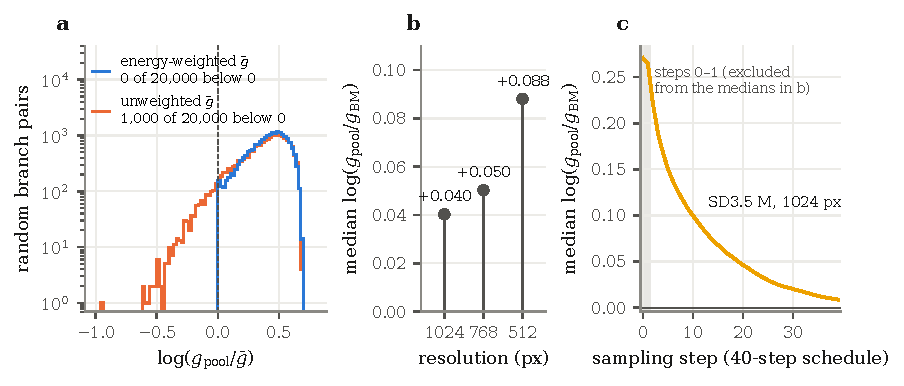
\includegraphics[width=\linewidth]{II-F2_pooling_theorem}
 \caption{\textbf{Pooling theorem and the capture functional.} Theorem: $\Phi(M)=(\operatorname{tr}M^{1/2})^2=D\,g(M)\operatorname{tr}M$ is concave and positively 1-homogeneous on the PSD cone. Hence for a pooled matrix $M=\sum_i\pi_iM_i$, $g_{\rm pool}\ \ge\ \sum_i\omega_i g_i$, with $\omega_i=\pi_i\operatorname{tr}M_i/\operatorname{tr}M$. That is, pooled $g$ is at least the \emph{energy-weighted} mean of the branch values. With equal branch energies this becomes $g_{\rm pool}\ge\overline{g_i}$. The weaker corollary $\sqrt{g_{\rm pool}}\ge\overline{\sqrt{g_i}}$ is what Round 5 Q1e tested, and it held in 100\% of (generation, step, layer) cells. The theorem does \textbf{not} give $g_{\rm pool}\ge$ the unweighted mean of $g_i$ in general. (a) Illustration: Monte Carlo over 20,000 random PSD branch pairs with unequal energies ($D=2$--32). Measured against the energy-weighted mean, there are 0 violations. Measured against the unweighted mean, 1,000 of the 20,000 pairs (5\%) fall below zero. (b) Identical-trajectory increments: the median $\log(g_{\rm pool}/g_{\rm BM})$ for steps $\ge2$ is $+0.040$, $+0.050$ and $+0.088$ at 1024, 768 and 512 px. This is SD3.5 Medium at CFG 4.5, with deterministic replay of the same generations (60, 29 and 29 pairs). The gap is unchanged ($|\Delta\log{\rm gap}|<3\times10^{-5}$). (c) The same increment by sampling step at 1024 px. It is largest at high $\sigma$ and decays along the schedule. The excess tracks the cond/uncond dissimilarity ($1-$prompt\_influence; Spearman 0.83, Q1f). Pooling therefore moves scalar $g$ without any change in the conditional trajectory. Source: Round 5 Q1c--Q1f (\texttt{review/round5/out/Q\_results.json}); register M5/T1.}
 \label{fig:pool}
\end{figure}

%=====================================================================
\section{Projection degeneracy and an equivalence hierarchy}\label{sec:hierarchy}

\subsection{Scalar envelopes are dominated by shared trends}
Let $P$ be any map from the trajectory $z(\cdot,\tau)$ to a scalar curve $a(\tau)$, for example the layer mean of $g$. Suppose two models share a monotone trend: $a(\tau)=\alpha_a T(\tau)+r_a(\tau)$ and $b(\tau)=\alpha_bT(\tau)+r_b(\tau)$ with $\alpha_a\alpha_b>0$.

\begin{proposition}[Trend dominance]\label{prop:trend}
Let $\alpha_aT+r_a$ and $\alpha_bT+r_b$ be the least-squares fits of $a$ and $b$ on $T$ over the sampled grid, with fitted slopes of the same sign, $\alpha_a\alpha_b>0$, so that $r_a$ and $r_b$ are exactly uncorrelated with $T$ on that grid,\footnote{Residuals that are merely independent of $T$ are not orthogonal to it on a finite grid, and sample correlations can then fall below the bound.} and write $\kappa_a=\operatorname{Var}(r_a)/(\alpha_a^2\operatorname{Var} T)$ and $\kappa_b$ likewise. Then
\begin{equation}
 \operatorname{corr}(a,b)\ \ge\ \frac{1-\sqrt{\kappa_a\kappa_b}}{\sqrt{(1+\kappa_a)(1+\kappa_b)}} .
\end{equation}
In particular $\operatorname{corr}(a,b)\to1$ as $\kappa_a,\kappa_b\to0$, whatever the residuals are.
\end{proposition}
\begin{proof}
$\operatorname{Cov}(a,b)=\alpha_a\alpha_b\operatorname{Var}T+\operatorname{Cov}(r_a,r_b)\ge\alpha_a\alpha_b\operatorname{Var}T-\sqrt{\operatorname{Var}r_a\operatorname{Var}r_b}$; divide by $\sqrt{\operatorname{Var}a\operatorname{Var}b}$ with $\operatorname{Var}a=\alpha_a^2\operatorname{Var}T(1+\kappa_a)$.
\end{proof}
The sign condition is on the fitted slopes, not on those of a generating model: noise can flip a weak fitted slope, and then the bound can fail (an explicit violation, $\operatorname{corr}=-0.27$ against a bound of $-0.02$, was constructed by a reviewer; filtering on the fitted slopes restores the bound in every draw). In the archive every envelope correlation is strongly positive, so the condition holds there. The bound is attained when the residuals are perfectly anti-correlated, $\operatorname{corr}(r_a,r_b)=-1$. When they are uncorrelated the correlation is $1/\sqrt{(1+\kappa_a)(1+\kappa_b)}$, above the bound, so the bound can be loose; it is a floor that holds for any residual dynamics, not an estimate. How binding it is depends on the trend chosen (post hoc, Mode-I RC25, layer-mean attention $g$ of the five archive campaigns on a common $\sigma$ grid). With $T$ linear in $\sigma$, $\kappa=0.10$--$4.0$ and the floor is weak for Mochi, whose envelope is not linear in $\sigma$. With $T$ the five-model mean envelope (which contains both models of a pair, so this is descriptive), $\kappa=0.01$--$0.36$, and the floor alone gives $0.61$--$0.95$ for the eight unrelated pairs, $0.005$--$0.18$ below their observed correlations (per-pair $\kappa$, floor and observed value in Supplement Table~\ref{tab:kappa}): on that grid the shared trend accounts for nearly all of each unrelated envelope correlation.

So a high envelope correlation is evidence of a shared trend, not of a shared mechanism; this is the classical problem of nonsense correlation between trending series \citep{yule1926why,granger1974spurious}, and a deterministic relative of the observation that identical summary statistics can hide different structure \citep{matejka2017same}. Every denoising trajectory in the archive shares a coarse trend in $\sigma$, so the envelope correlation of any two models is bounded below by a quantity that does not depend on their residual dynamics. In the data, all eight unrelated pairs have envelope correlations between $0.73$ and $0.98$ on linear $g$, and the best of them (Z-Image Turbo with SD3.5 Large, $r=0.981$) exceeds the pair formed by the same Turbo weights at 8 and 25 steps (\TT{}$\leftrightarrow$ZIT, $r=0.933$). With the real Base, an unrelated pair (Base with SD3.5 Medium, $0.982$) again exceeds Base$\leftrightarrow$Turbo ($0.964$; post hoc). The same unrelated pair has level-field correlation $0.48$, shape $0.46$ and tangent $-0.02$: a near-perfect envelope with no shared depth dynamics. Every attention envelope rises and then falls late in all five models, which supplies the shared trend.

\subsection{Four comparison levels: exact relations and graded statistics}
Let $\mathcal Z_m$ be the population field $\bar z_m(u,\tau)=\E_{p,s}z_{m,p,s}(u,\tau)$, defined on matched sampling states (equal $\sigma$; \S\ref{sec:tangent}). Define the standardised depth profile $\tilde z_m(\cdot,\tau)$ by $z$-scoring each of $(\log g,\log\gap,H)$ across depth at each $\tau$, interpolated to a common grid of 24 values of $u$.

\begin{definition}[Comparison levels]\label{def:levels}
For models $a,b$ at matched states $\tau$:
\begin{itemize}
 \item \textbf{envelope}: $\rho_{\mathrm{env}}=\operatorname{corr}_\tau\big(\bar g_a(\tau),\bar g_b(\tau)\big)$, on $g$ or $\log g$;
 \item \textbf{field}: $\rho_{\mathrm{field}}=\operatorname{corr}_{u,\tau}\big(\bar z_a,\bar z_b\big)$ on the level field;
 \item \textbf{shape}: $\rho_{\mathrm{shape}}=\E_\tau\operatorname{corr}_u\big(\tilde z_a(\cdot,\tau),\tilde z_b(\cdot,\tau)\big)$;
 \item \textbf{tangent}: $\rho_{\mathrm{tan}}=\E_\tau\cos\big(\Delta_u\tilde z_a(\cdot,\tau),\Delta_u\tilde z_b(\cdot,\tau)\big)$, with $\Delta_u$ the first difference along the depth grid.
\end{itemize}
\end{definition}

Write $a\sim_\bullet b$ for exact agreement at level $\bullet$ ($\rho_\bullet=1$) at every matched state. Then
\[
 a\sim_{\mathrm{field}} b\ \Rightarrow\ a\sim_{\mathrm{shape}} b\ \Longleftrightarrow\ a\sim_{\mathrm{tan}}b,\qquad a\sim_{\mathrm{field}}b\ \Rightarrow\ a\sim_{\mathrm{env}}b,
\]
for profiles in which every coordinate varies across depth (so that $z$-scoring is defined). Equal level fields have equal standardised profiles and equal layer means. Shape and tangent coincide as exact relations: equal standardised profiles have equal differences; conversely, $\rho_{\mathrm{tan}}=1$ at a state means that the concatenated difference vectors are positively proportional, $\Delta_u\tilde z_a=c\,\Delta_u\tilde z_b$ with $c>0$, so $\tilde z_a=c\,\tilde z_b+C$ coordinate by coordinate; zero depth mean forces $C=0$ and unit depth variance forces $c=1$. Without standardisation the tangent relation would be strictly weaker, since equal differences fix a profile only up to a constant. The first implication does not reverse: two fields can share standardised profiles and differ in layer means and scales. The four levels therefore differ as graded statistics rather than as exact classes. Correlating levels and correlating first differences weight depth frequencies differently: differencing multiplies the depth-frequency-$k$ component of an $n$-point profile by $2\sin(\pi k/2n)$, so the tangent down-weights slow depth trends and up-weights structure at the scale of a few layers. Two near-equal profiles can therefore score high on shape and low on tangent when they differ at layer scale, which is where unrelated models differ (Mode-I RC54: in the lowest quarter of depth frequencies unrelated pairs agree too, and the separation lies in the upper three quarters). Because that decomposition is of differences, which up-weight fast depth variation by construction, it describes how the estimator behaves, not a lineage mechanism, and it does not separate training relation from architecture. The canonical tangent statistic takes linear interpolation onto a depth grid of $n$ points, equal weight on the three coordinates and the nearest $\sigma$ of the second model; $z$-scoring across depth removes any depth-constant shift of $\log g$, in particular the width term $\log(D/D')$ of Lemma~\ref{lem:rot}(ii). Both papers lead with the native grid, $n$ equal to the number of hooked layers of the shallower model (24, 28 or 30), and give the preregistered $n=24$ beside it; the two coincide for 24-layer pairs. The native grid is the one size the sampling fixes. For $n$ below the layer count, linear interpolation is not an ideal low-pass filter: it drops the depth frequencies the coarse grid cannot represent and folds part of them back into those it can. A numerical reconstruction separates the two (Mode-I RC56): on 12 points the folded components carry $6$--$35\%$ of the difference energy, but removing them before resampling changes the tangent little (correlation $0.96$, largest change $0.17$), and unrelated attention pairs still rise to $0.49$--$0.65$, so the lost frequencies, not the folding, account for most of the lost separation. Above the layer count, added points are interpolants and carry no new information; at $n$ equal to the layer count of an equal-depth pair every recorded layer enters once. Its values depend on the grid (Mode-I \S5.3--5.4 and Table~9: tier values move by up to $0.25$ between 12, 24 and 48 points; related pairs lie above unrelated ones at 24 and 48 points, not at 12, where depth-matched unrelated pairs rise to $0.38$--$0.63$, and the order of the Z-Image siblings and the ACE-Step distillation pair flips between 12 and 48; on the native grid related pairs give $0.55$--$1.00$ and unrelated pairs $-0.17$ to $0.20$, with the Z-Image siblings at $0.55$ in attention, $0.25$--$0.27$ above both nulls; Mode-I RC30, RC33) and on the coordinate weighting (computed on one coordinate alone the order holds on $\log g$ and on $H$ in every lineage cell, and on the gap in three of four; Mode-I RC18). The empirical statistics are graded rather than exact, but the logic explains the observed ordering: coarse relations are easy to satisfy, and the tangent removes exactly the level and trend that Proposition~\ref{prop:trend} shows to be uninformative.

\subsection{What the coordinates cannot see}\label{sec:invariance}
Every comparison level is built from the triple $(g,\gap,H)$, so what the levels can detect is limited by what the triple ignores. The answer is exact.

\begin{lemma}[Invariance of the spectral triple]\label{lem:rot}
Let $X\in\R^{N\times D}$ have singular values $s_1\ge s_2\ge\dots\ge s_{\min(N,D)}\ge0$, with $\operatorname{rank}X\ge2$ so that $\gap$ is finite. Zero singular values are kept in $s$, with $0\log0=0$ in $H$; every statement below holds for rank-deficient $X$.
\begin{enumerate}
 \item[(i)] For $c>0$, $U\in O(N)$ (in particular any permutation of tokens) and $Q\in O(D)$, the matrix $cUXQ$ has the same $g$, $\gap$ and $H$ as $X$. The triple depends on $X$ only through the normalised spectrum $s/\sum_i s_i$, and two matrices of the same shape have the same normalised spectrum exactly when they are related in this way.
 \item[(ii)] If $V\in\R^{D\times D'}$ has orthonormal rows ($VV^\top=I_D$, $D\le D'$), then $\gap(XV)=\gap(X)$, $H(XV)=H(X)$ and $g(XV)=(D/D')\,g(X)$. Applied at every layer with the same ratio $D/D'$ (the same isometric embedding width at every depth), this shifts $\log g$ by the constant $\log(D/D')$, so the standardised profile $\tilde z$ and the tangent statistic are unchanged. If the width varies with depth, as across the levels of a U-Net ($320$--$1280$ channels), the shift is not constant and $z$-scoring does not remove it: the tangent is then not width-invariant, and Mode-I's U-Net check accordingly reports no tangent value.
 \item[(iii)] For a general invertible $A\in\R^{D\times D}$ the triple of $XA$ differs from that of $X$. Whitening, $A=M^{-1/2}$, flattens the spectrum: $g=1$ when $X$ has full column rank, and $g=\operatorname{rank}(X)/D$ in general when the whitening acts within the row space.
 \item[(iv)] Equal triples do not imply equal normalised spectra.
\end{enumerate}
\end{lemma}
\begin{proof}
(i) $UXQ$ has the singular values of $X$, and $g$, $\gap$ and $H$ are homogeneous of degree zero in $s$. Conversely, if $s(Y)=c\,s(X)$, writing both singular value decompositions gives $Y=cUXQ$. (ii) $(XV)(XV)^\top=XX^\top$, so $XV$ has the singular values of $X$ followed by $D'-D$ zeros. Zeros leave $\sum_i s_i$, $\sum_i s_i^2$, $s_1/s_2$ and $H$ unchanged; only the prefactor $1/D$ in (\ref{eq:g}) becomes $1/D'$. A constant added to $\log g$ at every depth is removed by $z$-scoring across depth, and so is not seen by $\tilde z$ or its depth difference. (iii) After whitening, $M=I$ (or the projector onto the row space), so all non-zero singular values are equal and the Cauchy--Schwarz bound of \S\ref{sec:observables} is attained. (iv) The normalised spectrum ranges over a simplex of dimension $\operatorname{rank}X-1$ and the triple fixes three functions on it. An explicit pair for $D=6$, given as a numerical certificate, is $s_a=(5,3,2.2,1.4,0.8,0.3)$ and $s_b=(5.077544162561188,\allowbreak\ 3.046526497536713,\allowbreak\ 1.488979904804269,\allowbreak\ 1.460983188909761,\allowbreak\ 1.442985275863451,\allowbreak\ 0.182980970324620)$: both give $g=0.6472830885303795$, $\gap=1.6666666666666667$ and $H=1.5172723029214925$ in double precision (the maximum difference is $0$; rounding $s_b$ to three decimals moves them by about $2\times10^{-4}$) and at equal $\sum_i s_i$ the spectra differ by $0.71$ in the largest elementwise difference ($L^\infty$); the normalised spectra $s/\sum_is_i$ differ by $0.13$ in $L^1$ and $0.056$ in $L^\infty$. The pair was found by matching the three equations (equal $g$, $\gap$ and $H$ at equal $\sum_is_i$, so six unknowns and four constraints) with Nelder--Mead from 400 random starts around $s_a$ and keeping the exact solution farthest from $s_a$ (\texttt{scripts/lemma\_rotation\_invariance.py}, part D), then polishing it by Gauss--Newton (\texttt{scripts/lemma9\_certificate.py}). The counterexample is not isolated: on the five-dimensional slice of equal $\sum_is_i$ the Jacobian of the triple at $s_b$ has rank three (singular values $0.632$, $0.226$, $0.049$ in the chart of the certificate script: the raw triple $(g,\gap,H)$ against an orthonormal basis of the five sum-zero directions; the values depend on that chart, the rank does not), so by the implicit function theorem the spectra near $s_b$ with the triple of $s_a$ form a smooth two-dimensional family; exact solutions are found at distances $0.01$--$0.1$ from $s_b$ along it, all at least $0.64$ from $s_a$ in $L^\infty$. Existence is all the lemma needs; the rank argument shows the gap between triple and spectrum is generic, not a numerical accident. How far apart two spectra with one triple can be, as a function of $D$ and of the triple, is an open problem; the certificate is existence evidence only.
\end{proof}

The lemma becomes informative once it is set against the symmetries of the networks themselves. In a pre-norm residual transformer, act on the residual stream by $h\mapsto hR$, with read weights $W\mapsto R^{-1}W$, write weights $W\mapsto WR$, embedding $E\mapsto ER$ and head $W_U\mapsto R^{-1}W_U$. If the normalisation satisfies $\operatorname{norm}(hR)=\operatorname{norm}(h)R$, the reparametrised network computes the same function, and every hooked block output written to the residual stream transforms as $X\mapsto XR$.

\begin{corollary}[Which symmetries the telemetry is blind to]\label{cor:rot}
\begin{enumerate}
 \item[(a)] With RMSNorm, after its gain is folded into the read weights, every $R\in O(D)$ is a symmetry. This is the computational invariance of \citet[Theorem~1]{ashkboos2024slicegpt}, and it applies to the autoregressive models in the archive. By Lemma~\ref{lem:rot}(i), two such weight settings give identical telemetry.
 \item[(b)] With LayerNorm acting on uncentred activations, $R\in O(D)$ is a symmetry exactly when $R\mathbf 1=\pm\mathbf 1$, which includes all channel permutations. Converting LayerNorm to RMSNorm, as \citet{ashkboos2024slicegpt} do, centres the stream and therefore changes the hooked activations.
 \item[(c)] With adaptive normalisation, where a conditioning-dependent per-channel scale multiplies the normalised stream \citep{peebles2023scalable}, $R$ must map every reachable diagonal scaling to a diagonal scaling. If the reachable modulations separate the channels (for every pair $i\neq j$ some conditioning gives $m_i\neq m_j$), the orthogonal matrices that do so are the signed permutations: no continuous rotation survives, and with LayerNorm the sign flips are lost as well. If some channels receive identical modulation under every conditioning, rotations within each such class survive.
 \item[(d)] Within this class, linear changes of residual basis that are compensated by the adjacent weights, a non-orthogonal invertible $A$ is a symmetry in none of these cases, because neither normalisation commutes with it. This is not a classification of all function-preserving reparametrisations of a network (for example, under an idealised scale-invariant normalisation without $\epsilon$, positive rescalings of the residual stream can be absorbed by the weights).
\end{enumerate}
\end{corollary}
\begin{proof}
(a) Right multiplication by an orthogonal $R$ preserves each token's norm, so $\operatorname{RMSNorm}(hR)=\operatorname{RMSNorm}(h)R$. (b) LayerNorm is RMSNorm applied after the centring projector $P=I-\mathbf 1\mathbf 1^\top/D$, and $PR=RP$ for orthogonal $R$ exactly when $R\mathbf 1=\pm\mathbf 1$. (c) The block computes $\operatorname{norm}(h)\operatorname{diag}(1+m)W$ with a modulation $m$ that varies with conditioning. Invariance requires $R\operatorname{diag}(1+m)R^{\top}$ to be diagonal for every reachable $m$. Conjugation is linear, so this holds exactly when $RSR^\top$ is diagonal for every $S$ in the linear span $\mathcal S$ of the reachable matrices $\operatorname{diag}(1+m)$; the condition is on $\mathcal S$. If the reachable modulations separate channels $i$ and $j$, so does $\mathcal S$; and since a finite union of proper subspaces cannot cover $\mathcal S$, a generic element $G\in\mathcal S$ then separates every separated pair at once. When every pair is separated, $G$ has distinct diagonal entries, its eigenvectors are the coordinate axes, and $RGR^\top$ diagonal forces each row of $R$ to be an eigenvector of $G$, that is $\pm$ a coordinate vector: $R$ is a signed permutation. When some channels are never separated, every element of $\mathcal S$ is constant on those classes, and any rotation within a class leaves it unchanged, so rotations within classes survive (whatever else $\mathcal S$ contains); further $R$ may survive depending on $\mathcal S$. Separation by the reachable modulations is the condition, and it is equivalent to separation by their span: an affine modulation $m=Wc+b$ of even a one-dimensional conditioning $c$ separates channels unless two rows of $(W,b)$ coincide, so the richness assumption holds generically for real AdaLN layers. The archive does not log modulation statistics, so that the learned rows are distinct in the archive's models is an assumption about trained weights, not a measurement. For a signed permutation, relabelling the modulation outputs by $|R|$ restores the function. (d) $\|hA\|\neq\|h\|$ in general. All four cases are checked numerically on toy two-block networks in \texttt{scripts/lemma\_rotation\_invariance.py} (with generic, channel-separating modulations), which also checks (i)--(iv) of the lemma (39 of 39 checks as expected; \texttt{data/II-lemma\_rotation\_check.csv}).
\end{proof}
Three groups should be kept apart: the transformations that preserve the spectral triple (Lemma~\ref{lem:rot}(i): scalings, token permutations and every $Q\in O(D)$); the residual-basis changes that commute with a given normalisation (Corollary~\ref{cor:rot}); and all function-preserving reparametrisations of a network, a larger set that the corollary does not classify. The telemetry is blind to the intersection of the first two. Case (c) rests on an assumption about trained weights that the archive does not measure, so for the archive's models it is conditional. Table~\ref{tab:symclass} places the models of the archive in these cases.

\begin{table}[h]
\centering\small
\caption{Corollary~\ref{cor:rot} applied to the models in the archive, by the normalisation each uses on the hooked residual stream (as described in their releases).}
\label{tab:symclass}
\begin{tabularx}{\linewidth}{@{}lLL@{}}
\toprule
Case & Models & Rotations the telemetry cannot detect\\
\midrule
(a) RMSNorm & language-model controls (Qwen2.5, Qwen3.5, Llama~3.1, Mistral, Gemma~3) & all of $O(D)$, one shared across depth\\
(b) LayerNorm, unmodulated & none in the archive & channel permutations and $R$ with $R\mathbf 1=\pm\mathbf 1$\\
(c) adaptive (timestep) modulation & Z-Image, SD3.5 Medium and Large, SD3 Medium, Mochi~1, ACE-Step~1.5, PixArt-$\Sigma$, Cosmos-Predict2 & signed permutations (permutations only with LayerNorm)\\
not covered & SD1.5 U-Net (convolutions, GroupNorm, varying width) & no continuous symmetry of this form\\
\bottomrule
\end{tabularx}
\end{table}


\begin{remark}[What tangent agreement does and does not say]\label{rem:rot}
The lemma gives one direction only. Suppose the hooked activations of two models are related at every matched $(u,\tau)$ by $X_b=c\,U X_a Q$, with rotations that may differ from layer to layer. Then their fields agree at every level of Definition~\ref{def:levels}. By (ii), the same holds across different widths after an isometric embedding, so width alone cannot produce a low tangent value (for example, for SD3.5 M$\leftrightarrow$L or the Qwen sizes).

The converse fails twice. First, equal triples do not fix the spectrum, by (iv). Second, equal spectra fix the activations only up to an independent rotation at each layer. The network's own symmetry, by contrast, is a single rotation shared across depth, and it exists only in case (a).

High tangent agreement, such as the same-weights $0.94$--$0.999$ or the lineage and sibling pairs $0.55$--$0.93$ (native grid), is therefore a necessary condition for an orthogonal correspondence of the two models' activations. It is not evidence for one. It says that the two models move three rotation-invariant functionals of the spectrum in the same direction along depth, at matched states. This is the precise sense in which \S\ref{sec:tangent} calls the relation a partial correspondence in the measured coordinates. Every comparison in these coordinates, the identity gate of Mode-I included, is blind to function-preserving rotations of case (a) and to the signed permutations of case (c). Sufficiency would need information the triple discards: the full singular-value spectrum at each layer (which closes the first gap), and the activations themselves or the weights, from which an orthogonal map between the two models can be fitted and tested directly, for example by orthogonal Procrustes or CKA on stored activations, or by aligning weights up to the network's symmetry group. Mode-I's Round 18 stored coarse per-layer activation sketches for this baseline on the same pairs (addendum B, \S\ref{sec:tangent}): on them the preregistered CKA statistic does not reproduce the tangent's separation of related from unrelated pairs, so a full-resolution test of sufficiency is still open.

A related gap separates states from their derivatives. If a map $\phi$ satisfies $\phi(\bar z_a(u,\tau))\approx\bar z_b(u,\tau)$ on a set of landmarks, then $D\phi\,\partial_u\bar z_a\approx\partial_u\bar z_b$ is an additional constraint, implied only when the landmarks are dense along trajectories and $\phi$ is fitted on their tangent bundle. Aligned states with unaligned derivatives are therefore possible, and \S\ref{sec:tangent} shows that they are common across architectures.
\end{remark}

\subsection{Data anchor}
Define the margin of a pair at each level as its value minus the best unrelated pair. On the archive (Round 6, preregistered S1) the campaign pair whose files are labelled Base and Turbo is the same Turbo weights at 8 and 25 steps (\TT{}$\leftrightarrow$ZIT). The real Base$\leftrightarrow$Turbo row was computed afterwards with the same functions on the real Base conditional branch (Z1), against the eight archive unrelated pairs plus Base against Mochi and SD3.5 M and L (post hoc), so its unrelated set differs from the Round 6 row's:
\begin{center}\small
\begin{tabular}{lccccc}
\toprule
Margin & linear $g$ & $\log g$ & field & shape & tangent\\
\midrule
Same weights, \TT{}$\leftrightarrow$ZIT (R6, preregistered) & $-0.049$ & $+0.047$ & $+0.131$ & $+0.152$ & $+0.703$\\
Lineage, Base$\leftrightarrow$Turbo (post hoc) & $-0.018$ & $+0.003$ & $+0.036$ & $+0.060$ & $+0.496$\\
\bottomrule
\end{tabular}
\end{center}
The same-weights tangent is $0.94$--$0.999$ and every unrelated pair is at most $0.24$; that value is unchanged on 60-generation subsets (5--95\% within $0.01$ of the full value; Round 8 R8-13). The real lineage tangent is $0.707$ (attention) and $0.719$ (MLP) on the preregistered 24-point grid, and the best unrelated pair involving Base or Turbo is $0.21$ (Round 12, preregistered); on the native 30-point grid the pair, siblings within one family, gives $0.547$ and $0.771$ (Mode-I RC33). In both rows the margin increases monotonically with the stringency of the relation, and only the tangent separates the pair clearly; the lineage margins are smaller at every level (Fig.~\ref{fig:controls}a).

\begin{figure}[t]
 \centering
 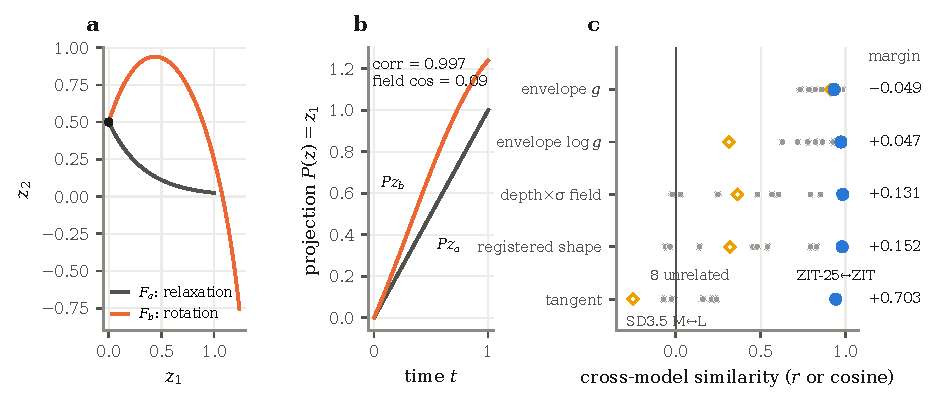
\includegraphics[width=\linewidth]{II-F3_projection_degeneracy}
 \caption{\textbf{Projection degeneracy and the equivalence hierarchy.} (a,b) Illustration: two different planar fields, $F_a$ (drift plus relaxation) and $F_b$ (drift plus rotation). Their trajectories from the same start have scalar projections $P(z)=z_1$ that correlate at $0.997$, while the centred fields have cosine $0.09$ over the plotted domain. A high correlation of a one-dimensional projection does not identify a shared vector field. (c) Measured cross-model similarity at five observable levels (Round 6 S1, preregistered). Shown are \TT{}$\leftrightarrow$ZIT, the same Turbo weights at 25 and 8 steps (blue), the eight unrelated pairs (gray) and SD3.5 M$\leftrightarrow$L (open diamond). Its margin over the best unrelated pair rises with the observable: $-0.049$ (scalar envelope $g$), $+0.047$ ($\log g$), $+0.131$ (depth$\times\sigma$ field), $+0.152$ (registered shape) and $+0.703$ (tangent). On the scalar curve, ZIT$\leftrightarrow$SD3.5 L (0.981) exceeds \TT{}$\leftrightarrow$ZIT (0.933). The real Base$\leftrightarrow$Turbo lineage is in Fig.~\ref{fig:controls}a. A scalar envelope correlation therefore cannot identify lineage, or even the same weights, when every envelope shares a monotone trend (register T2). The statement concerns similarity by correlation. A supervised classifier trained on spectral responses can still tell models apart \citep{meshram2026diffusion}; what the shared trend removes is the ability of a high correlation to signal shared mechanism or descent. Source: \texttt{review/round6/out/S1\_hierarchy.csv}.}
 \label{fig:hier}
\end{figure}

%=====================================================================
\section{A non-autonomous flow family}\label{sec:flow}

\subsection{The model class}
The natural dynamical reading of the archive treats depth as time, as in the ODE view of residual networks and transformers \citep{e2017proposal,lu2018beyond,lu2019understanding,chen2018neural,geshkovski2025mathematical}, and asks for a vector field
\begin{equation}\label{eq:flow}
 \partial_u z = F_m(z,u,\tau),
\end{equation}
which in discrete form is the layer step $\beta(u,\tau)=z(u+\Delta u,\tau)-z(u,\tau)$. Two simpler classes are tempting and both fail.
\begin{itemize}
 \item \emph{Autonomous scalar law} $\beta_g=F(g)$. The cloud of $(g,\beta_g)$ points pools all layers and steps; its zero crossings are not fixed points of a one-dimensional flow, because the same $g$ is visited at different $(u,\tau)$ with different $\beta$. Section~\ref{sec:nulls} shows that the crossings of the pooled cloud are partly reproduced by surrogates that keep only marginals or the mean field.
 \item \emph{Autonomous state law} $\partial_uz=F(z)$ with $z=(g,\gap,H)$. Under held-out prediction with flexible learners, once normalised depth $u$ and clock $\tau$ are supplied the full state adds a median of only $0.014$ in $R^2$ (about $0.032$ in diffusion channels and $0.010$ in fixed-context autoregressive channels; D08). Under the frozen minimal-sufficiency rule, 7 of 12 channels need only $(u,\tau)$ and the other 5 need only $(g,u,\tau)$ (D09). The rule takes the smallest of the nested sets $(u,\tau)\subset(g,u,\tau)\subset(g,\gap,H,u,\tau)$ whose held-out $R^2$ comes within a fixed tolerance of the full feature set; every accepted set is within $0.018$ of the full $R^2$ and every rejected set falls short by at least $0.030$ (reproducer \texttt{D09\_minimal\_coordinate\_set.py}, ledger).
\end{itemize}
These two results are close to true by construction: when the system$\times$time scaffold holds $96\%$ of the variance (\S\ref{sec:family}), a state that lies on that manifold adds little once its coordinates $(u,\tau)$ are known. We read D08 and D09 as a statement about how the measured manifold is parametrised, and rest the non-autonomy argument on the transfer results below (D03, D15), which are not tautological. The full $R^2$ ladder is in Fig.~\ref{fig:closure} of the Supplementary material, annotated accordingly.
The flow is therefore explicitly non-autonomous \citep{kloeden2011nonautonomous}: most of the predictable structure is carried by where and when, not by the current spectral state. The same holds in the SD1.5 U-Net and in the distilled ACE-Step checkpoint, where a block or layer effect adds a held-out $\Delta R^2$ of $0.46$--$0.77$ to a spline in $g$ (preregistered), and in the undistilled ACE-Step Base for the MLP ($0.671$) but not for attention ($0.254$, where $g$ alone already predicts the depth step; Mode-I \S12), so non-autonomy is checkpoint-dependent in attention.

\subsection{Preferred decomposition}
We write
\begin{equation}\label{eq:decomp}
 \partial_u z = F^{(0)}_m(u,\tau) + R_m(z,u,\tau),
\end{equation}
an anatomical drift $F^{(0)}_m$ (the population mean field's derivative) plus a state-dependent residual $R_m$. Within a model the decomposition predicts well: prompt-held-out state-plus-coordinate $R^2$ is $0.941$--$0.987$ (D03).

\subsection{Transfer across models}
The decomposition does not transfer across architectures. A vector field fitted on one model and applied to Mochi or SD3.5 Medium or Large after dimensionless normalisation gives $R^2$ near zero or negative (D03). Removing the scaffold $F^{(0)}$ and fitting only the residual $R$ does not help: residual transfer between the same Turbo weights at 25 and 8 steps (\TT{}$\leftrightarrow$ZIT) averages $R^2=0.437$ against a target-self ceiling of $0.579$, while unrelated transfers average $-0.256$ against ceilings near $0.459$ (D15). Direct \TT{}$\leftrightarrow$ZIT transfer of the full field remains substantial ($R^2=0.70$--$0.75$ in attention, $0.72$--$0.89$ in MLP). Most unrelated pairs in D15 differ in depth, so the failure could be a depth artefact. A re-implementation of the D15 design on depth-matched pairs (post hoc, Mode-I RC24; gradient-boosted residual field on standardised $(\log g,\log\gap,H)$, scaffold removed, prompt-grouped self ceiling) rules that out. Unrelated pairs at equal depth (PixArt-$\Sigma$$\leftrightarrow$Cosmos, ACE-Step$\leftrightarrow$SD3 and SD3.5 Medium) give a mean cross-model $R^2$ of $-0.33$ against self ceilings of $0.28$; Z-Image Turbo in two sessions transfers at its ceiling (shortfall $\le0.06$); and the real distillation pairs fall in between (shortfall $0.37$). The ACE-Step turbo session pair loses $0.23$--$0.25$ in attention, the capture-session effect of Mode-I \S12.2. Against a same-weights prompt-split null every unrelated and lineage shortfall is beyond chance and the successor's is not (RC28; Finding~\ref{fd:nofield}). Reparameterising progress by cumulative spectral arc length raises unrelated correlations by only $+0.057$ on average and the preregistered paired test is not significant ($p\approx0.105$; D17, Supplement~\ref{app:arclength}).

\begin{table}[htbp]
\centering\small
\caption{Residual vector-field transfer after scaffold subtraction (D15; gradient-boosted regression on the residual state, attention unless marked). Self: the target's own held-out $R^2$ (its ceiling). Cross: $R^2$ of the field fitted on the source and applied to the target.}
\label{tab:transfer}
\begin{tabular}{llccc}
\toprule
Source $\to$ target & Relation & Self & Cross & Shortfall\\
\midrule
ZIT $\to$ \TT{}, \TT{} $\to$ ZIT (attn) & same weights & 0.49, 0.52 & 0.36, 0.40 & 0.14, 0.12\\
ZIT $\to$ \TT{}, \TT{} $\to$ ZIT (MLP) & same weights & 0.67, 0.64 & 0.50, 0.48 & 0.16, 0.15\\
SD3.5 M $\to$ L, L $\to$ M & scaling pair & 0.45, 0.32 & 0.09, $-0.14$ & 0.36, 0.46\\
ZIT $\to$ Mochi, Mochi $\to$ ZIT & unrelated & 0.38, 0.60 & $-0.15$, $-0.50$ & 0.53, 1.10\\
ZIT $\to$ SD3.5 M, SD3.5 M $\to$ ZIT & unrelated & 0.37, 0.64 & $-0.59$, $-0.24$ & 0.96, 0.88\\
\bottomrule
\end{tabular}
\par\smallskip\footnotesize Shortfalls are computed from unrounded $R^2$ values, so they can differ by $0.01$ from the difference of the printed columns.
\end{table}

\begin{finding}[Fitted residual fields do not transfer in these coordinates]\label{fd:nofield}
Within the model class \eqref{eq:flow} evaluated on $z=(g,\gap,H)$ and normalised $(u,\tau)$, a residual field fitted on one model and applied to a different checkpoint falls short of the target's own ceiling by more than the same-weights null in every unrelated pair and every distillation pair tested at matched depth (shortfall $0.28$--$1.35$ unrelated, $0.23$--$0.56$ lineage; every bootstrap 5th percentile above the pooled null 95th percentile; post hoc, RC28). The archive pairs of Table~\ref{tab:transfer}, which differ in depth, agree ($0.36$--$1.10$ against $0.12$--$0.16$ for the same weights). The same-vendor successor SD3 Medium$\leftrightarrow$SD3.5 Medium stays within the null (shortfall $0.02$--$0.03$), with a self ceiling of only $0.11$--$0.12$.
\end{finding}
\paragraph{Error statement (post hoc, RC28).} The null is built from the same weights. For each target model, 20 random prompt halves are drawn; the residual field is fitted on one half and applied to the other, and the null shortfall is the target's self $R^2$ minus the $R^2$ on the held-out half. Fitting on half the prompts makes this null conservative: it overstates the shortfall the same weights would show. Pooled over the ten targets, its 95th percentile is $0.167$ in attention and $0.098$ in MLP (per model $0.036$--$0.256$). For each depth-matched pair of Mode-I RC24 the target's prompts are resampled 200 times, and a pair counts as beyond the same weights if the 5th percentile of its shortfall exceeds the pooled 95th percentile, a one-sided test at about $5\%$ per pair. All 8 unrelated and all 8 lineage pair-directions pass, the closest by $0.06$ (ACE-Step turbo$\to$Base, attention, 5th percentile $0.226$); both successor directions and the Z-Image session pairs do not. Two caveats. The ACE-Step turbo session pair also exceeds the pooled threshold in attention ($0.23$--$0.25$), although it is within ACE-Step turbo's own null ($0.256$): its attention field varies strongly across prompts, and against that model-specific null one lineage direction (Base$\to$turbo, $0.255$) no longer passes. And the shortfall does not order the tiers: the lineage and unrelated ranges overlap. The finding is therefore a test of ``same weights'' against ``different checkpoint'' in these coordinates, not a lineage measure, and for the successor pair, whose ceiling is low, it has little power. The direct (non-residual) transfers into Mochi and SD3.5 (D03) were recorded in the ledger only as ``approximately zero or negative'', without per-pair values, and are not used. It is an empirical finding about these coordinates and about the pairs tested, not a theorem. A shared field could exist in other coordinates or in a quotient; \S\ref{sec:universality} discusses what that would require.


%=====================================================================
\section{The trajectory family and its neighbourhoods}\label{sec:family}

For descriptive purposes we write
\begin{equation}\label{eq:gamma}
 z_{m,p,s}(u,\tau)\ \approx\ \Gamma_m(u,\tau)+\delta_{m,p}(u,\tau)+\varepsilon_{m,p,s}(u,\tau),
\end{equation}
a model scaffold $\Gamma_m$, a deterministic content modulation $\delta_{m,p}$ and a stochastic seed term $\varepsilon_{m,p,s}$. The terms are defined by nested conditional means, not as orthogonal effects: in an unbalanced archive the variance shares depend on the order of conditioning, and the system and time rows are nested components rather than ANOVA main effects.

Two statements hold together and must be reported together (D12):
\begin{itemize}
 \item Across the whole archive the system$\times$time scaffold accounts for $96.2\%$ of normalised depth-geometry variance (and $95.6\%$ of absolute operating-point variance); theme, prompt and seed share the remaining $3.8\%$.
 \item Within a fixed (model, state) cell, prompt identity explains $51\%$ to $96\%$ of the variance as a naive share, and $36\%$ to $95\%$ after correcting for seed replication in a random-effects decomposition; the lowest values are at $\sigma=1$ in \TT{}, whose pooled first step carries a large seed share.
\end{itemize}
The first is a statement about how different models and sampling states are; the second says that, once those are fixed, the content term $\delta$ is the dominant source of variation. The deterministic content geometry (\S\ref{sec:content}) and the stochastic seed neighbourhood (\S\ref{sec:estimators}) are therefore different objects and are analysed separately.

\begin{figure}[t]
 \centering
 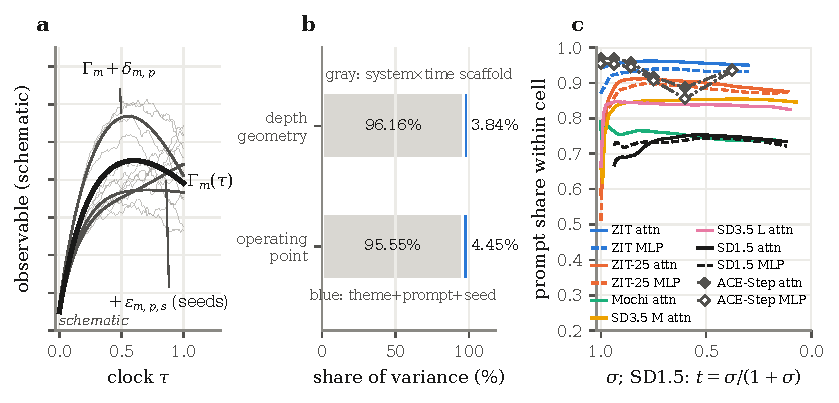
\includegraphics[width=\linewidth]{II-F5_trajectory_decomposition}
 \caption{\textbf{Trajectory decomposition $M_{m,p,s}(\tau)\approx\Gamma_m(\tau)+\delta_{m,p}(\tau)+\varepsilon_{m,p,s}(\tau)$.} (a) Schematic: a model backbone $\Gamma_m$, prompt modulations $\delta_{m,p}$ and seed neighbourhoods $\varepsilon_{m,p,s}$. The components are descriptive and not orthogonal. (b) Nested variance split (ledger D12). The system$\times$time scaffold holds 96.16\% of normalized depth-geometry variance (theme+prompt+seed 3.84\%) and 95.55\% of the absolute operating point (4.45\%). Most of the 96\% is between-model and between-time variance. (c) Within a fixed (model, sampling-state) cell, prompt identity is the largest component. The naive between-prompt share is 0.51--0.96 across seven archive channels and all $\sigma$ (Round 2 E6; the ANOVA seed-corrected share is 0.36--0.95). \TT{}'s share is lowest at $\sigma=1$, where its archive capture is pooled, so part of that dip may come from the capture regime. Mochi CFG 1, with one seed per prompt, is omitted. Black (post hoc): the SD1.5 U-Net of Mode-I, conditional branch, plotted against the rectified-flow clock at equal signal-to-noise ratio, $t=\sigma/(1+\sigma)$; its naive share is 0.67--0.75 (ANOVA 0.56--0.67), inside the archive range. Diamonds (post hoc): the audio model ACE-Step (turbo), 0.86--0.97 (ANOVA 0.82--0.96), with no early rise (B10 refuted); in the undistilled ACE-Step Base the ANOVA share rises first (0.34$\to$0.46 attention, 0.22$\to$0.41 MLP; B10 holds, Round 14, not drawn). State both numbers (register \#14). Sources: ledger D12; \texttt{review/round2/out/E6\_varcomp\_by\_step.csv}.}
 \label{fig:family}
\end{figure}

%=====================================================================
\section{Tangent agreement within a lineage}\label{sec:tangent}

\subsection{Registration}
Z-Image Turbo is a few-step model distilled within the Z-Image family: its technical report distils ``our foundational SFT model'' with Decoupled DMD and DMDR (\citealp[\S4.5 and Fig.~13]{zimageteam2025zimage}; \citealp{liu2025decoupled}); Z-Image Base is the released undistilled model of the same family \citep{tongyi2026zimage}. ACE-Step~1.5 likewise ships a distilled turbo checkpoint (released for 8 steps at shift 3; captured at 6, and at 8 in Mode-I's Round 16) and an undistilled Base \citep{gong2026acestep15}; which checkpoint served as turbo's teacher is not documented in the material we used. We call each a lineage pair; the word names the relation, not the mechanism, and the design cannot separate the distillation objective from shared pretraining, data and text encoder. Mode-I's Round 17 shows that a same-vendor successor that is not a distilled student (SD3 Medium$\leftrightarrow$SD3.5 Medium; whether it continues SD3 Medium's training is not documented) reaches the same tier, so lineage is meant in that broad sense. Within Z-Image, all captures use a flow-matching schedule at shift $3.0$, so states are matched by equal $\sigma$. On the archive, equal-$\sigma$ matching is within $0.005$ in registered correlation of the optimised affine warp, per prompt it loses at most $0.011$ (and at most $0.01$ in 99\% and 100\% of prompts for attention and MLP; R1, R2), and every prompt chooses zero layer shift (117 of 117). Those checks compared the same Turbo weights at 25 and 8 steps (\TT{}$\leftrightarrow$ZIT), so they show that a step-count change does not compress the clock; they say nothing about a lineage. The real Base comparisons below also use equal $\sigma$ (nearest state, Round 6 estimator unchanged), with the registration fixed in the preregistration rather than fitted.

\subsection{The tangent statistic: tiers}
With registration fixed, the tangent statistic $\rho_{\mathrm{tan}}$ of Definition~\ref{def:levels} measures whether two models take the same direction in standardised spectral coordinates as depth increases. Mode-I (\S5.3--5.5) reports the values; we summarise only what the theory needs. Mode-I separates what is measured, related depth-matched pairs far above their nulls and unrelated pairs at or barely above them (at 24 grid points or finer; not at 12), from a finer three-tier ordering among the related pairs that it reads as a hypothesis to be revisited, since the boundary between same weights and a close relative is not established and the order of the two distillation families changes with the grid (Mode-I Table~9). A documented teacher--student pair at equal depth, SD3.5 Large against SD3.5 Large Turbo (adversarial diffusion distillation, 38 blocks each), was preregistered as Mode-I Round 18 to test it and lands in the middle tier: $0.818$ on the 24-point grid and $0.904$ on the native grid, $0.58$ above its permutation null, below the same weights across sessions ($0.998$) and level with the same-vendor successor. The three tiers as read: the same weights under changed inference give $0.94$--$0.999$, and the capture functional alone accounts for most of the shortfall from one (Theorem~\ref{thm:pool}); the two lineage pairs give $0.71$/$0.72$ on the 24-point grid ($0.55$/$0.77$ native; Z-Image, a sibling pair) and $0.80$/$0.59$ (ACE-Step at its release setting of 8 steps, attention/MLP, Round 16; the original 6-step measurement gave $0.85$/$0.57$), the ACE-Step MLP value carried by the last layers; and the one depth-matched unrelated pair, ACE-Step against SD3.5 Medium, gives $-0.07$ to $-0.11$, inside its null. On Z-Image image rows the attention lineage value rises to $0.93$, within $0.07$ of same weights (post hoc). Three later rounds, frozen before their captures (Mode-I Rounds 16--18), narrow this. ACE-Step at its release setting of 8 steps gives $0.80$/$0.59$, and the same turbo weights in two capture sessions give $0.92$/$0.82$, so same weights is not one number. SD3 Medium against SD3.5 Medium, a same-vendor successor rather than a distilled student, gives $0.926$ in attention, in the middle tier and level with same weights across sessions. A depth-matched unrelated image pair, PixArt-$\Sigma$ against Cosmos-Predict2 2B, gives $0.303$ in attention, just above its null, but $0.687$ in MLP, inside the lineage range and carried mostly by the last block. In attention the tangent therefore grades relatedness, without a sharp line between the same weights and a close relative; in MLP its bottom tier does not hold, with or without the end layers (post hoc, Mode-I RC22). A layer-order permutation destroys depth smoothness, so it can understate how often smooth unrelated profiles agree. Against a smoothness-preserving surrogate, in which the second model's depth-difference profile is phase-randomised with one phase vector shared by all states and coordinates, every related pair stays above the 95th percentile by about $0.25$ or more, the cross-modal unrelated pairs fall inside it, and at most $5\%$ of surrogate draws reach the lineage rule (Mode-I RC22). Same weights across capture sessions give $0.98$--$1.00$ in Z-Image and SD3.5 Medium, so the ACE-Step session value is the exception, not the rule; SD3.5 Large across sessions gives $0.998$ (Round 18). Round 18 also found that a second capture session at the same prompts, seed and settings replays the first exactly, so a session change alone adds no variation, and that Base at its official shift $6.0$ gives the same sibling value ($0.520$/$0.760$ native against $0.547$/$0.771$ at shift 3). Three language-model families give no attention pair outside the unrelated range, but one same-vendor MLP pair (Qwen3.5$\leftrightarrow$Qwen2.5) reaches $0.66$ against a layer-permutation 95th percentile of $0.32$ (R15-6), so the tangent is a screen whose false-positive rate is unknown, not a detector: the depth-matched unrelated values on file are five model pairs of two types, none above the lineage rule, which bounds the false-positive rate at $78\%$ (two types) or $45\%$ (five pairs) with 95\% confidence (Mode-I RC53). The related pairs also share more architecture than the unrelated ones, so architecture and training relation are not separated; a same-architecture, independently trained control is a Mode-III test.

\paragraph{Depth calibration.} The tangent takes first differences of profiles interpolated to a common grid. For an equal-depth pair the native grid reads every layer once; for pairs of unequal depth no grid does so for both models. Differencing is a high-pass operation, so structure at the scale of single layers maps onto the grid differently at different depths, and the statistic is not invariant under a change of depth. Empirically (Mode-I \S5.4), a model against a depth-subsampled copy of itself keeps $0.90$--$0.99$ when the copy has 24 layers but falls to $0.08$--$0.81$ at other depth ratios (Mode-I \S5.4), while smoothing across depth restores self-copies only by lifting unrelated pairs to $0.5$--$0.84$. A depth-invariant version would need a reparametrisation of depth that both models share, which the triple does not supply (Lemma~\ref{lem:rot} concerns the activations at one layer, not the correspondence between layers). Every same-weights and lineage pair is depth-matched, and of the unrelated pairs only ACE-Step against SD3.5 Medium and PixArt-$\Sigma$ against Cosmos are, so the tiers are a statement about depth-matched pairs, and cross-depth tangents are not calibrated levels.

\subsection{State alignment does not align derivatives}
One can ask whether unrelated models would also agree once their state spaces are aligned. Procrustes, linear and CCA maps fitted on state landmarks without derivative labels visibly improve state alignment between unrelated fields, but the matched depth derivatives remain near zero or anti-aligned: the best mapping for each unrelated pair averages a derivative correlation of $0.007$, while the same Turbo weights at 25 and 8 steps (\TT{}$\leftrightarrow$ZIT) average $0.937$ across mappings and channels (D10). D10 has not been recomputed on the real Base captures. This is the empirical counterpart of the last paragraph of Remark~\ref{rem:rot}: aligned states with unaligned derivatives are common across architectures and absent within one set of weights. An activation baseline points the same way (Mode-I \S5.7, Round 18 addendum B, preregistered). On stored activation sketches (36 image tokens per hook, four states), symmetric best-match linear CKA ranks related above unrelated pairs well (AUC $0.968$) but puts every pair, related or unrelated, above its prompt-permutation null and does not separate the Z-Image siblings ($0.344$) from the highest unrelated pair ($0.364$), while the attention tangent separates the same depth-matched pairs by $0.33$; secondary variants separate them post hoc by $0.01$--$0.05$. This coarse baseline (36 float16 tokens, four states) therefore does not reproduce what the depth derivative separates, at three scalars per layer and step; a clean float32 comparison is a Mode-III test. There is an exact theoretical instance of the same gap: at large $N$ a chaotic nonlinear random recurrent network has the same covariance matrix as a stable linear network with the same couplings driven by independent noise \citep{shen2025covariance,clark2026linear}, so equal second-moment geometry coexists with opposite Lyapunov behaviour, and the stability of the dynamics has to be read from the tangent dynamics themselves \citep{clark2026lyapunov}.

\subsection{Interpretation}
The relation between a distilled checkpoint and its source is a partial, orientation-preserving correspondence of trajectories in the measured coordinates, at equal $\sigma$ and equal depth, and it is clearly weaker than the relation of one checkpoint to itself under changed inference. It is weaker than topological conjugacy or orbit equivalence \citep{katok1995introduction}: it holds for the projected flow, not for the hidden state, and only at the sampled states. In Z-Image, distillation lowered $g$ at every layer by enlarging a shared mean direction, and changed the first and last layers more than layers 17--22 (Round 13, split-half preregistered, 6 of 6 Z-Image predictions held); in ACE-Step the direction of the $g$ change is not consistent across layers (14 and 10 of 24; Round 14). On the archive, the MLP local eigenmode sequence is closed by a geometry-derived 25$\to$8-step registration ($p=0.002$) but attention is not ($p=0.26$); that test compared the same Turbo weights and has not been repeated on the real Base (\S\ref{sec:linear}). The contemporary distillation literature aligns depth trajectories rather than single layers \citep{chi2026mta}; our measurements show that trajectory agreement within the model families tested can be detected without access to the training objective, at a strength that differs between families and submodules; whether it tracks the training relation or shared architecture is open.

\begin{figure}[t]
 \centering
 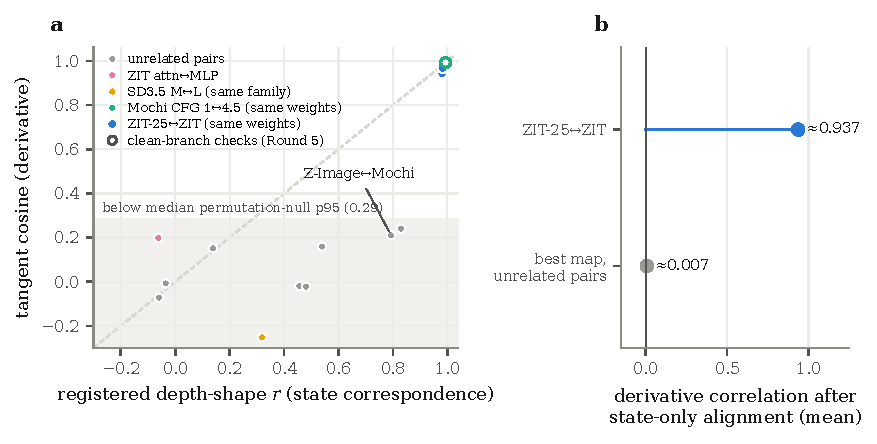
\includegraphics[width=\linewidth]{II-F6_tangent_inheritance}
 \caption{\textbf{Tangent-field agreement: state correspondence is not dynamics correspondence.} (a) Registered depth-shape $r$ against the depth-derivative (tangent) cosine at matched $\sigma$ for 13 channel pairs (Round 2 E10). Every Z-Image pair here is the same Turbo weights: the blue pair is \TT{}$\leftrightarrow$ZIT. The open markers are Round 5 clean-branch checks: \TT{} CFG 4 cond-branch$\leftrightarrow$ZIT: 0.992 attention, 0.992 MLP; \TT{} CFG 1$\leftrightarrow$CFG 4: 0.991 and 0.993. Unrelated pairs reach a shape $r$ of up to 0.83 (Z-Image$\leftrightarrow$Mochi), yet their tangent cosine stays $\le0.24$, inside each pair's permutation null (the shaded band is the median null p95, 0.29). \TT{}$\leftrightarrow$ZIT scores 0.94--0.97 and the same-weights Mochi CFG pair 0.99. The real Base$\leftrightarrow$Turbo lineage (0.71/0.72, Round 12) is not drawn here; see Fig.~\ref{fig:controls} and Mode-I Fig.~14. SD3.5 M$\leftrightarrow$L, a scale change within one family, scores $-0.25$. (b) Ledger D10: state-only alignment maps (Procrustes, linear, CCA) are fitted without derivative labels. After them, matched derivative correlation averages $\approx0.937$ for \TT{}$\leftrightarrow$ZIT and $\approx0.007$ for the best map of each unrelated pair. Aligning representations does not align their dynamics. Sources: \texttt{review/round2/out/E10\_tangent.csv}, \texttt{review/round5/out/Q\_results.json} (Q2a, Q2c), ledger D10.}
 \label{fig:tangent}
\end{figure}

\begin{figure}[t]
 \centering
 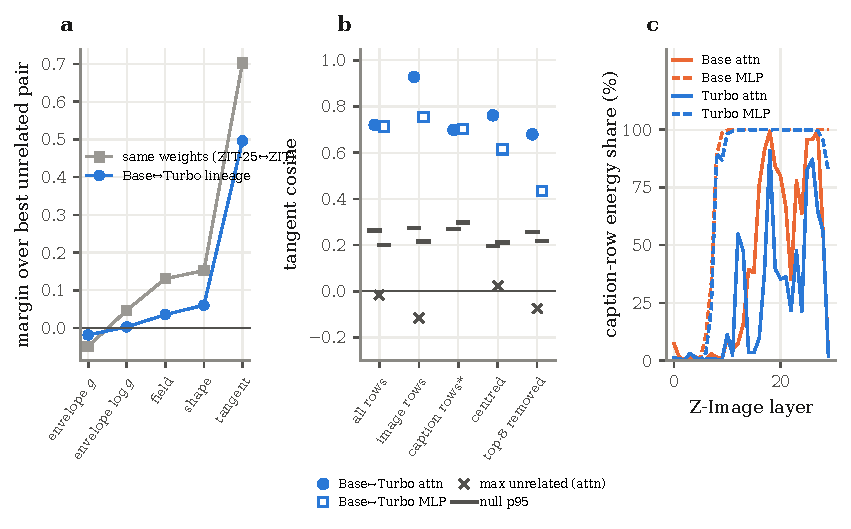
\includegraphics[width=\linewidth]{II-F13_lineage_controls}
 \caption{\textbf{The real lineage pair under the uncentred-statistic controls.} (a) Margin over the best unrelated pair at the five levels of Definition~\ref{def:levels} (attention). Gray: the same Turbo weights at 25 and 8 steps (\TT{}$\leftrightarrow$ZIT; Round 6 S1, preregistered): $-0.049$ to $+0.703$. Blue: the real Z-Image Base (conditional branch)$\leftrightarrow$Turbo, same functions, post hoc: $-0.018$, $+0.003$, $+0.036$, $+0.060$ and $+0.496$. Both rise with the stringency of the relation; only the tangent separates the lineage clearly. (b) Round 11 (preregistered; caption rows post hoc): Base$\leftrightarrow$Turbo tangent per row-split variant, attention (filled) and MLP (open), with layer-permutation null p95 (dark ticks) and the largest unrelated value (Base or Turbo against SD3.5 Medium, attention; crosses). All rows $0.72$/$0.71$; image rows $0.93$/$0.75$; caption rows $0.70$/$0.70$; centred $0.76$/$0.61$; eight largest channels removed $0.68$/$0.43$; unrelated $-0.13$ to $0.02$. (c) Median share of the uncentred second-moment energy carried by the 64 caption rows of the joint sequence, by layer (60 prompts, CFG 1, conditional branch). In MLP it is at least $98\%$ in every layer from 10 to 26 in both models (layers 8--9 are transitional, and Turbo's last three layers fall to $0.71$--$0.91$); in attention it varies between $3\%$ and $100\%$ in the second half of the network. Sources: \texttt{review/round6/out/S1\_results.json}; \texttt{review/zib\_turbo\_mixup\_2026-10-18/r12/out/posthoc\_hierarchy\_margins.csv}; \texttt{review/peer\_review\_2026-10-17/r11/out/}; row-split cubes \texttt{V\_Z2\_*.pkl}, \texttt{V\_ZITSV\_*.pkl}.}
 \label{fig:controls}
\end{figure}

%=====================================================================
\section{Content geometry is a different quotient}\label{sec:content}

For a set of prompts $\{p_1,\dots,p_n\}$ shared by two models, let $\Delta_m(\tau)\in\R^{n\times n}$ be the matrix of distances between prompt-mean profiles of model $m$ at state $\tau$. The representational similarity between models is the Spearman correlation of the upper triangles of $\Delta_a$ and $\Delta_b$, tested by a Mantel permutation \citep{mantel1967detection,kriegeskorte2008representational}. Mantel tests have lower power than raw-data tests and are biased under autocorrelation \citep{legendre2010comparison,guillot2013dismantling}, which is why we also permute within themes and partial out text distances. Two prompts are equivalent in this quotient if they occupy the same relative positions, whatever the absolute geometry.

Mode-I (\S6.2) reports the values: the prompt-relational structure is shared across all five diffusion models (Mantel $\rho=0.13$--$0.43$ between unrelated models, $0.56$--$0.62$ for the same weights; preregistered), within themes, beyond text and length, and on image-only and centred rows (post hoc). Within the Z-Image lineage the attention value ($0.61$--$0.67$) overlaps the same-weights range, so content geometry does not tier by lineage, while the depth tangent drops to the middle tier; in ACE-Step the lineage content geometry does not replicate (R15-3), and domain decoders do not transfer across families, so shared geometry is not shared coordinates. Comparisons are at each model's recommended operating point, on which prompt RSA depends (Fig.~\ref{fig:content}, Supplement~\ref{app:supp}). The sharing is therefore not a restatement of the prompt list.

Across the ten model pairs with both measurements, the Spearman correlation between first-state content similarity and tangent similarity is $0.297$ ($p=0.405$). With ten pairs this test has little power; we read it as no detectable rank coupling, not as independence. The two quotients nevertheless behave differently: content relations are shared broadly across unrelated models and are strongest for the same weights, while tangent agreement separates same weights, lineage and unrelated models into tiers.



%=====================================================================
\section{Two sign-topology constructions}\label{sec:topology}

The archive supports two different ``three-phase'' statements. They live on different axes and must not be merged.

\subsection{Along the sampling clock}
Let $\bar g(\tau)=\E_{u,p,s}\,g(u,\tau)$ be the layer-mean $g$ of a submodule, and call its three-segment sign pattern the clock-axis sequence, fitted by a piecewise-linear model with two breakpoints and scored by its bootstrap rate and a time-order permutation null. In Mode-I (\S7.1) the sequence $+,-,+$ holds for Z-Image Turbo MLP only, and there only on all rows: it disappears on image rows, centred and pruned statistics, so it is a property of Turbo's caption-row MLP statistic, and real Base, attention, the U-Net and ACE-Step do not show it.

\subsection{Along depth}
Define the layer step of $g$ at fixed $\tau$, $\beta_\ell=g(\ell+1)-g(\ell)$, and bin the cloud of $(g,\beta)$ points into 29 bins in $g$ (at least 10 points per bin); the sign pattern of the binned mean $b(g)=\E[\beta\mid g]$ and its zero crossings are the CoS-PAFS analyzer's layer-flow measurement. The cloud pools all $(p,s,\ell,\tau)$, so a zero crossing is a property of the conditional mean $\E[\beta\mid g]$, not a fixed point of a one-dimensional flow (\S\ref{sec:flow}). Mode-I (\S7.2) reports where the three-crossing pattern $+,-,+,-$ appears: in several archive channels, with different surrogate classes, at some $\sigma$ in every archive architecture, but not in the real Z-Image Base conditional branch or in either ACE-Step checkpoint; the same Turbo weights show or lose it with step count, guidance and capture, and in SD3.5 Medium it disappears when the activations are centred. It is a property of model and capture functional, and, where tested, of the uncentred moment (Fig.~\ref{fig:topology}, Supplement~\ref{app:supp}).

\subsection{Null classes}
Two surrogate families decide what part of the pattern is generic (\S\ref{sec:nulls}): Surrogate A permutes each layer's $g$ across all rows (keeps per-layer marginals); Surrogate B permutes $g$ across generations within each (layer, step) cell (keeps the mean field $\bar g(\ell,\tau)$). In SD3.5 Medium attention and in 25-step Turbo attention and MLP (\TT{}) neither surrogate reproduces the pattern (0 of 1000 draws each; Mode-I RC14), so it needs within-generation layer coupling. In 8-step Turbo MLP it beats Surrogate A but is reproduced by Surrogate B: it follows from the mean field. In SD3.5 Large it is reproduced by both (null-generic).

\subsection{Why crossing ratios are not invariants}
The crossing locations $g^*_1<g^*_2<g^*_3$ and the interval ratio $(g^*_2-g^*_1)/(g^*_3-g^*_1)$ vary from $3\%$ to $77\%$ across channels. They depend on the capture functional (Theorem~\ref{thm:pool} shifts every $g$), on which submodules are pooled, on which steps are mixed into the cloud, and on the sample size (20 versus 480 generations change the crossing count). None is an invariant. What is robust is the sign sequence together with its bootstrap rate and surrogate class, reported per channel.



%=====================================================================
\section{Kinematic nulls and surrogate theory}\label{sec:nulls}

\subsection{The differencing null}
The archive also records $\varphi$, the cosine between successive layer displacements of the activations. Its raw value clusters near $-1/2$, which has a trivial explanation.

\begin{proposition}\label{prop:diff}
Let $x_1,x_2,x_3\in\R^D$ be independent with common mean $\mu$ and covariance $\Sigma$, and $d_1=x_2-x_1$, $d_2=x_3-x_2$. Then $\operatorname{Cov}(d_1,d_2)=-\Sigma$ and $\operatorname{Cov}(d_i,d_i)=2\Sigma$, so each coordinate pair has correlation $-1/2$. If in addition the $x_i$ are Gaussian and $\Sigma$ has effective rank growing with $D$ ($\tr\Sigma^2/(\tr\Sigma)^2\to0$), then $\cos(d_1,d_2)\to-1/2$ in probability, with fluctuations of order $(\tr\Sigma^2)^{1/2}/\tr\Sigma$. For the stride-two pair $d_1=x_2-x_1$, $d_3=x_4-x_3$, which share no term, $\operatorname{Cov}(d_1,d_3)=0$ and $\cos(d_1,d_3)\to0$.
\end{proposition}
\begin{proof}
$\operatorname{Cov}(x_2-x_1,x_3-x_2)=-\operatorname{Var}(x_2)=-\Sigma$. For the cosine, write $y_i=x_i-\mu$, so $d_1=y_2-y_1$, $d_2=y_3-y_2$, $\E d_1^\top d_2=-\tr\Sigma$ and $\E\|d_i\|^2=2\tr\Sigma$. In the Gaussian case Isserlis' theorem gives the variances: $d_1^\top d_2=y_2^\top y_3-y_1^\top y_3-\|y_2\|^2+y_1^\top y_2$, whose four terms are pairwise uncorrelated, with variances $\tr\Sigma^2$ for each cross term and $2\tr\Sigma^2$ for $\|y_2\|^2$, so $\operatorname{Var}(d_1^\top d_2)=5\tr\Sigma^2$; and $d_i\sim N(0,2\Sigma)$, so $\operatorname{Var}\|d_i\|^2=2\tr(2\Sigma)^2=8\tr\Sigma^2$. Dividing by $\tr\Sigma$, the numerator and both squared norms concentrate at $-1$ and $2$ with standard deviations $O\big((\tr\Sigma^2)^{1/2}/\tr\Sigma\big)\to0$, and the continuous mapping theorem gives $\cos(d_1,d_2)\to-1/2$. The stride-two pair shares no term, so its numerator has mean zero and the same concentration gives $0$.
\end{proof}
For non-Gaussian $x_i$ the same conclusion holds whenever the quadratic forms concentrate, for instance when $y=x_i-\mu=\Sigma^{1/2}w$ with $w$ having independent sub-Gaussian coordinates, where the Hanson--Wright inequality \citep{rudelson2013hanson} gives $|y^\top Ay-\E y^\top Ay|=O_P(\|\Sigma^{1/2}A\Sigma^{1/2}\|_F)$ for each fixed $A$, and $\|\Sigma^{1/2}A\Sigma^{1/2}\|_F^2=O(\tr\Sigma^2)$ for the bounded matrices $A$ that write $d_1^\top d_2$ and $\|d_i\|^2$ as quadratic forms in the stacked vector; the Gaussian proof then goes through unchanged. Without such an independence structure we state it as a remark. A raw $\varphi\approx-1/2$ is therefore what independent layers would give and carries no information about rotation. After null correction, $\varphi$ residuals reproduce between the same Turbo weights at 25 and 8 steps (\TT{}$\leftrightarrow$ZIT), but adding $\varphi$ to $[g,\gap,H,u,\sigma]$ adds no held-out predictive information (R2 P9), so $\varphi$ is redundant with depth and clock in this archive.

\subsection{Surrogates for the pooled cloud}
Surrogate testing rejects a specific null, not a mechanism \citep{theiler1992testing,schreiber2000surrogate,lancaster2018surrogate}; with trending data the null must preserve the trend \citep{nakamura2005small,harris2020nonsense}. We therefore use nulls that each keep one named component of the data.

A cloud-$\beta$ zero crossing is a statement about the binned conditional mean $\E[\beta\mid g]$ over all $(p,s,\ell,\tau)$. Each surrogate destroys one source of structure:
\begin{itemize}
 \item Surrogate A (layer marginals): permute $g$ within each layer across all generations and steps. Destroys every trajectory; keeps $\{g\mid\ell\}$.
 \item Surrogate B (mean field): permute $g$ across generations within each $(\ell,\tau)$ cell. Destroys within-generation coupling across layers; keeps $\bar g(\ell,\tau)$ and its spread.
\end{itemize}
If a crossing survives Surrogate A, it is produced by the per-layer distributions alone; if it survives B, it is produced by the population mean field, i.e.\ by the temporal profile folded into $(g,\beta)$. Only a crossing that both surrogates fail to reproduce requires trajectory-level coupling. A crossing reproduced by a surrogate is \emph{null-generic} under that construction and cannot be read as a fixed point or phase boundary of any dynamics.

\begin{figure}[t]
 \centering
 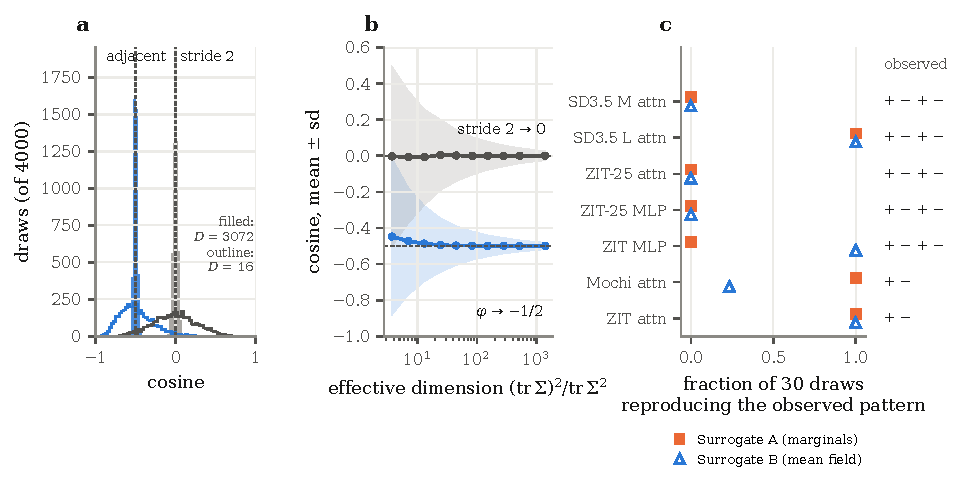
\includegraphics[width=\linewidth]{II-F9_differencing_nulls}
 \caption{\textbf{Differencing and surrogate nulls.} Let $v_k$ be i.i.d. with a common mean and covariance $\Sigma$, and let $d_k=v_{k+1}-v_k$. Then $\mathbb{E}[d_k\!\cdot\!d_{k+1}]=-\operatorname{tr}\Sigma$ and $\mathbb{E}|d_k|^2=2\operatorname{tr}\Sigma$. So the adjacent-difference cosine $\varphi$ concentrates at $-1/2$, and the stride-2 cosine at $0$, as the effective dimension $(\operatorname{tr}\Sigma)^2/\operatorname{tr}\Sigma^2$ grows. (a) Illustration: Monte Carlo distributions at $D=3072$ (filled) and $D=16$ (outline), with a power-law $\Sigma$. (b) Illustration: mean $\pm$ sd against effective dimension. At $D=3072$ (effective dimension 1390), $\varphi=-0.500\pm0.020$ and the stride-2 cosine is $0.000\pm0.027$. A raw $\varphi\approx-1/2$ is the null value, not a signal (register \#9, T4). (c) Post hoc analyzer replay A4. For each channel, the plot gives the fraction of 30 draws of the 09-15 Surrogate A (per-layer marginals) and Surrogate B (mean field $g(L,\sigma)$) that reproduce the observed whole-run $\beta_{\rm layer}$ pattern. A crossing that its surrogate reproduces is null-generic and is not a phase boundary. Source: \texttt{review/round6/out/A4\_beta\_layer\_surrogates.csv}.}
 \label{fig:nulls}
\end{figure}

%=====================================================================
\section{Local linearisation}\label{sec:linear}

Locally in depth we fit
\begin{equation}
 z(\ell+1)=A\,z(\ell)+b
\end{equation}
by least squares on windows of layers at fixed $\tau$, with $z=(g,-\gap,H)$, and record the eigenvalues of $A$. The gap enters with a minus sign so that all three coordinates increase as the spectrum flattens ($g$ and $H$ rise, the gap falls); the eigenvalues of $A$ do not depend on this choice or on a common change of units, a per-coordinate affine rescaling $z\mapsto Sz+c$ applied to every layer alike (it maps $A$ to the similar matrix $SAS^{-1}$), but the signs of its off-diagonal entries do. Rescalings that differ between the two sides of the map, or a reweighted least-squares refit, give a different $A$, not a similar one. This is a descriptive linear model in the spirit of dynamic mode decomposition and local linearisation of network dynamics \citep{schmid2010dynamic,williams2015datadriven,kutz2016dynamic,sussillo2013opening}; it does not claim that the underlying network is linear.

\begin{itemize}
 \item \emph{Complex pairs are not a signal.} Across start, middle and end states and across semantic domains, many cells have no complex eigenpair at all; the fraction ranges from 0 to 1 depending on architecture and state. Under a layer-order permutation null (one permutation per draw applied to every generation of a cell, 200 draws), complex pairs are more common ($67\%$ of fits) than in the data ($17\%$ of cells; post hoc, Mode-I RC23D), so the observed complex pairs are not evidence of rotation beyond what rough profiles produce.
 \item \emph{The dominant modulus is stable (descriptive, no null).} The modulus of the dominant eigenvalue is much more stable: its median coefficient of variation across domains is about $2\%$ ($2.2\%$ in the original census, $1.6\%$ in the re-implementation behind Fig.~\ref{fig:linear}; the figure plots the re-implementation because its per-domain values are released with the figure's data table). The modulus is below one almost everywhere; the exception is the first state of Z-Image MLP, where it is $1.03$--$1.23$. Theme explains about $17\%$ of contraction-modulus variation but only $0.8\%$ of rotation angle and $1.7\%$ of complex-mode occurrence (D07).
 \item \emph{A registration closes MLP modes within one model.} The geometry-derived 25$\to$8-step registration of the same Turbo weights (\TT{}$\to$ZIT) closes the MLP local eigenmode sequence ($p=0.002$ against all $8!$ time permutations) but not attention ($p=0.26$). It has not been repeated on a real lineage pair.
\end{itemize}
The same null was computed for the modulus: the data's dominant modulus lies above the permutation 95th percentile in $95\%$ of cells ($0.38$--$1.15$ against null medians of $0.19$--$0.36$), which is what smooth depth profiles produce, since a stable linear fit is expected for any slowly varying profile. The modulus is therefore a smoothness statistic of the depth profiles, and its recurrence is not evidence of a relaxational mechanism; the earlier reading of a rotational component that depends on architecture and state is retired. A null that keeps smoothness (as in Mode-I RC22) is the test that could still give the local maps content. An earlier study on legacy-instrument files found a stable complex pair with modulus $0.40$--$0.53$ on a terminal ``rebound'' branch of SD3.5 Medium; because those files were measured with a hook that substitutes a different attention path, we report it only in Appendix~\ref{app:legacy}.

\begin{figure}[t]
 \centering
 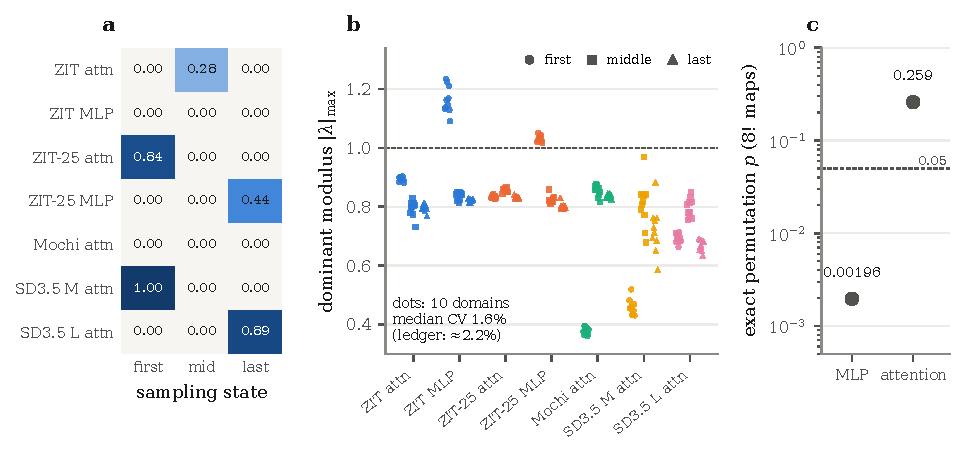
\includegraphics[width=\linewidth]{II-F10_local_mode_census}
 \caption{\textbf{Local linear mode census.} (a,b) The affine layer map $X_{L+1}=AX_L+b$ on $X=[g,-{\rm gap},H]$ is fitted per channel $\times$ sampling state (first, middle, last step) $\times$ semantic domain. Its eigenvalues are invariant to a common per-coordinate affine change of units. This is a \textbf{re-implemented estimator}, not the ledger's script 14, recomputed from the raw archive cubes. (a) The fraction of 100 generation bootstraps in which $A$ has a complex-conjugate pair, averaged over the 10 domains. It ranges from 0 to 1 depending on architecture and state. (b) The dominant modulus $|\lambda|_{\max}$, one dot per domain. The median across-domain coefficient of variation is 1.6\% here (ledger, script 14: $\approx2.2\%$). The modulus is below 1 in most cells but above 1 at the first state of Z-Image MLP. (c) Ledger, script 12: a \TT{}$\to$ZIT time warp (the same Turbo weights at 25 and 8 steps) is chosen from depth geometry alone. Under it, the local complex-mode sequence closes for MLP (exact permutation $p=0.00196$ over all $8!$ maps) but not for attention ($p=0.259$). Under a layer-permutation null complex pairs are more frequent ($67\%$) than in these fits ($17\%$), and the modulus exceeds the null in $95\%$ of cells, which smooth profiles produce (post hoc, Mode-I RC23D). This is descriptive and is no evidence of a physical oscillator or probability current. Sources: raw cubes; ledger cards "Complex local modes are regime-specific\ldots{}" (script 14) and "Geometry-derived Base$\to$Turbo warp\ldots{}" (script 12; the ledger's ``Base'' is \TT{}).}
 \label{fig:linear}
\end{figure}

%=====================================================================
\section{Estimators for seed predictability}\label{sec:estimators}

Let $r_{g,t}$ be the seed residual of generation $g$ at step $t$: the standardised state with the prompt mean removed. For each $t$ let $A(t)$ be the prompt-grouped cross-validated $R^2$ of a ridge map from $r_{\cdot,t}$ to the final residual $r_{\cdot,T-1}$. Then $A(T-1)$ is the predictability ceiling.

\paragraph{Threshold crossing depends on the ceiling.} The usual onset, $\sigma_{50}$, is the $\sigma$ at which $A(t)$ first exceeds $0.5$. Because ridge $R^2$ is biased downward in small samples, the ceiling $A(T-1)$ rises with the number of generations $n$ (in the explicit-branch captures from $0.48$ to $0.89$ as $n$ goes from 60 to 480), and so does any absolute threshold crossing: $\sigma_{50}$ is undefined in 98\% of partitions at $n=60$ and moves from $0.72$ to $0.94$ as $n$ grows. At matched $n$ across the Round 6 channels its range is $0.501$.

\begin{definition}[Relative onset]
$\sigma_{\mathrm{rel}}$ is the $\sigma$ at which $A(t)/A(T-1)$ first exceeds $1/2$, interpolated linearly in $\tau$.
\end{definition}
Normalising by the ceiling removes the first-order dependence on $n$. The threshold $1/2$ is a convention: at $0.3$, $0.4$, $0.6$ and $0.7$ the onsets move as any crossing rule's do, while the order of the seven channels is kept (Spearman $0.96$--$1.00$ with the $1/2$ order for $0.3$--$0.6$, $0.82$ at $0.7$; Mode-I RC20). At matched $n$, the range of $\sigma_{\mathrm{rel}}$ across channels is $0.277$, and its uncertainty interval is narrower than that of $\sigma_{50}$ in 7 of 7 channels (preregistered S3).

\paragraph{Variance ratios need a calibrated reference.} For a residual path $r_t$ define
\begin{equation}
 \mathrm{VR}(q)=\frac{\E\|r_{t+q}-r_t\|^2}{q\,\E\|r_{t+1}-r_t\|^2}
\end{equation}
\citep{lo1988stock}. For a random walk $\mathrm{VR}(q)=1$; for an i.i.d.\ sequence (whose increments are then $MA(1)$) $\mathrm{VR}(q)=1/q$; for a stationary AR(1) with coefficient $\phi$, $\mathrm{VR}(q)=(1-\phi^q)/(q(1-\phi))$. On short paths the sample statistic is biased below its population value \citep{kim1991mean,lo1989size}, and with per-step standardisation the bias is large: simulated paths of the archive's length give $\mathrm{VR}(4)\approx0.82$ for a random walk (not 1), $0.72$ for AR(0.8) and $0.25$ for an i.i.d.\ sequence. The estimator uses overlapping differences, $\widehat{\mathrm{VR}}(q)=\overline{\|r_{t+q}-r_t\|^2}/(q\,\overline{\|r_{t+1}-r_t\|^2})$ with means over generations and all admissible $t$, after dropping the first state, and no Lo--MacKinlay bias correction; the references are simulated at each channel's own (generations, steps, layers) shape and passed through the same residualisation and estimator (Round 6 S3), so a different estimator gives different reference values (a naive estimator on a 25-step walk gives about $0.88$). We therefore report $\mathrm{VR}(4)$ as a fraction of the simulated finite-walk value. The seed residuals sit at $0.49$--$0.87$ of the walk reference. AR(0.8) sits at $0.85$--$0.88$ on that scale, so most channels ($0.49$--$0.65$) are more mean-reverting than AR(0.8) and only Mochi ($0.85$) and SD3.5 Large ($0.87$) reach it; Z-Image Turbo attention is the exception at $1.13$. That exception is the value an 8-state path gives: subsampled to Turbo's 8 states, three of five 25--40-step channels exceed one (Round 8 R8-2).

\paragraph{What these estimators do not say.} A rising $A(t)$ means that the final seed residual becomes gradually more predictable from the current one. It is not a committor $q(x)$ \citep{e2010transitionpath}: no continuation from a fixed intermediate state was cloned and scored, so no statement about a fate boundary follows (\S\ref{sec:open}).

\begin{figure}[t]
 \centering
 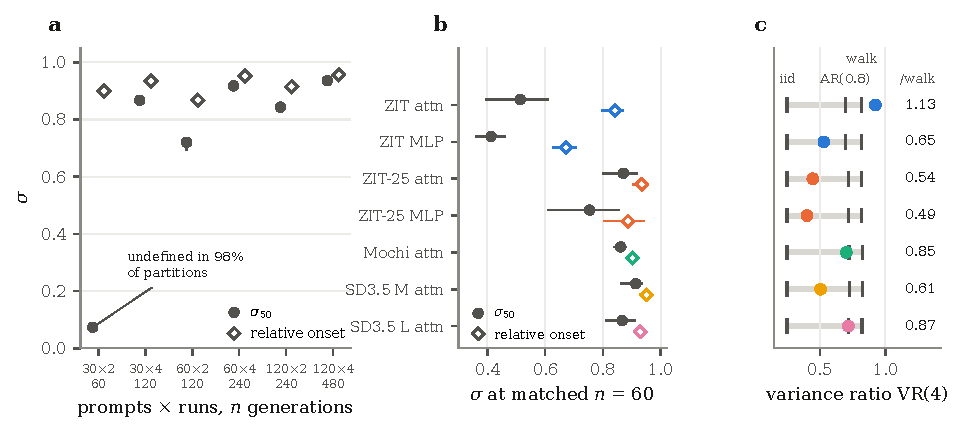
\includegraphics[width=\linewidth]{II-F11_estimators}
 \caption{\textbf{Estimator mathematics for seed predictability.} (a) $\sigma_{50}$ is a threshold crossing: the first $\sigma$ at which the cross-validated $R^2$ from state to final state passes 0.5. It therefore moves with the $R^2$ ceiling and with sample size. On nested subsets of the SD3.5 M archive (branch-mean capture), $\sigma_{50}$ goes from undefined (in 98\% of partitions) at $n=60$ to 0.94 at $n=480$. The relative onset on the same curves stays between 0.87 and 0.96. Bars are p5--p95 over fold partitions. (b) At matched $n=60$, across all seven archive channels, relative onset is 0.84--0.95 in six channels and 0.67 in ZIT MLP (8-step grid). Its range across channels is 0.28, against 0.50 for $\sigma_{50}$ (S3a--c). (c) The variance ratio VR(4) of seed-deviation residuals, against finite-length references simulated at each channel's own length (i.i.d. $\approx0.25$, AR(1) 0.8 $\approx0.72$, random walk $\approx0.82$). VR(4)/walk is 0.49--0.87 in six channels and 1.13 in ZIT attention. On the calibrated scale most channels sit below the AR(0.8) reference ($\approx0.85$--$0.88$ of walk); only Mochi and SD3.5 L reach it (S3d refuted the walk-like prediction). These panels calibrate estimators only. They make no claim about commitment or a separatrix (gate G3). Sources: \texttt{review/round5/out/H1\_seedfate\_vs\_sample\_size.csv}, \texttt{review/round6/out/S3\_estimators.csv}; register \#26--27.}
 \label{fig:estimators}
\end{figure}

%=====================================================================
\section{What kind of universality remains possible?}\label{sec:universality}

The fitted residual fields of \S\ref{sec:flow} do not transfer between the tested checkpoints, so no common field of that model class is supported in the present coordinates; a common law under other observation maps, hidden variables or coordinates is not excluded (Finding~\ref{fd:nofield}). The structure that does recur across unrelated architectures is coarser:
\begin{enumerate}
 \item \emph{coarse envelope recurrence}: shared trends in the sampling clock, an early high-speed transient at $\sigma\approx1$ followed by a $\sigma$-invariant plateau whose onset lies at $\sigma=0.78$--$0.87$ in eight channels of four families (at a fixed sampling shift; it moves with resolution); the depth sign sequence $+,-,+,-$ appears at some $\sigma$ in every archive architecture but not in the real Z-Image Base conditional branch or either ACE-Step checkpoint, so it is a property of model and capture, not a recurrent invariant (\S\ref{sec:topology});
 \item \emph{shared content geometry}: prompt-relational structure that persists within themes and beyond text overlap (\S\ref{sec:content});
 \item \emph{tiered tangent dynamics}, with only its coarse split measured: agreement of $\partial_uz$ at matched state separates related from unrelated depth-matched pairs; as a hypothesis, it is near one for the same weights under changed inference and intermediate within a lineage pair (native grid: ACE-Step distillation $0.57$--$0.85$; the Z-Image siblings $0.55$/$0.77$, and on image rows $0.91$ in attention, close to the successor; $0.93$ for a same-vendor successor that is not a distilled student), and in attention absent or weak between unrelated models ($-0.17$ to $0.20$; up to $0.30$ on the 24-point grid); shown for depth-matched pairs. In MLP an unrelated image pair reaches $0.57$ ($0.69$ on 24 points), so the MLP tangent does not tier (\S\ref{sec:tangent}).
\end{enumerate}
Two out-of-family checks in Mode-I (\S11--12) bound these items: a convolutional U-Net shares items~1 and~2 but not the degree of anisotropy or the clock-axis envelopes, and an audio flow transformer, in a distilled and an undistilled checkpoint, keeps the backbone and the plateau, loses the depth sign sequence in both checkpoints, and repeats item~3 as a second lineage tier. Several finer properties differ between the two audio checkpoints, so they are checkpoint-specific. Any universality statement consistent with the archive must therefore be one of: an invariance of ordering or topology (a sign sequence with its surrogate class), an equivalence in a quotient (content relations, or a reparameterisation of progress, though arc length fails; Supplement~\ref{app:arclength}), or an equivalence class under a family of projections.

A strong universality claim, one stated for whole trajectories and independent of the capture, would have to meet at least these conditions: (i) be stated for a capture functional that is fixed across models, or be invariant under the pooling map of Theorem~\ref{thm:pool}; (ii) survive Surrogates A and B in every channel it names; (iii) predict held-out models' tangent fields, not only their envelopes; (iv) be robust to removing the few dominant activation channels that drive uncentred spectra \citep{sun2024massive,turri2026few}, and to centring (Round 11: the Z-Image lineage tier survives both, the SD3.5 Medium depth sequence survives channel removal but not centring); and (v) hold for a submodule measured in every architecture (among the image transformers, the archive has MLP hooks only for Z-Image; the U-Net and audio checks have them); (vi) hold across data modalities and across checkpoints of one model, which the depth sign sequence does not; (vii) be computed on the rows that the claim is about: in joint text--image sequences, any future MLP universality claim must use image rows, not the caption rows that carry the uncentred energy; and (viii) be calibrated for depth mismatch, either by comparing depth-matched models or with an estimator shown to be invariant on depth-resampled copies of one model.

All eight are necessary for that strong form; none is sufficient alone, and together they are the minimum, not a guarantee. Necessary here means necessary for a claim to be about the models rather than about the capture. Weaker claims need fewer. A claim about a marginal or projected statistic, or one restricted to an architecture, needs the validity conditions that apply to the statistic it names, not the scope conditions: a property of the uncentred mean direction is not required to survive centring, only to say that it is about that direction, and a pattern reproduced by a mean-field surrogate can be a genuinely shared population property that simply does not show trajectory-level coupling. For joint text--image sequences, (vii) is blocking for any claim about image content: a value computed on all rows describes the caption rows wherever they carry the energy. Conditions (iv) and (vii) read like methodological preferences, but for this instrument they are not: the uncentred triple is a statistic that a few channels or rows can dominate (Mode-I Table~7), so without them a number may describe those channels or rows rather than the model. That some candidates cannot meet the list jointly is a finding about those candidates, not a defect of the list. They are not jointly satisfiable for every candidate claim: a statistic that depends on the uncentred mean direction, such as the SD3.5 Medium depth sequence, survives channel removal but not centring, so it cannot meet (iv) in full however it is captured. They are of two kinds (Table~\ref{tab:conditions}). Conditions (i), (ii), (iv), (vii) and (viii) are validity conditions: without them a cross-model number does not measure what it names. Conditions (iii), (v) and (vi) are scope conditions: they decide how far a valid result extends. The table marks which can be met from the existing archive and which need new captures. The next captures in this programme (Mode-III) take up (i), by restricting every cross-campaign comparison to conditional-branch captures, and (viii), by adding depth-matched unrelated pairs, since those two undercut the most tables.

\begin{table}[htbp]
\centering\small
\caption{The eight conditions of a universality claim: kind, and what the existing archive can and cannot satisfy.}
\label{tab:conditions}
\begin{tabularx}{\linewidth}{@{}lllL@{}}
\toprule
 & Condition & Kind & Existing archive\\
\midrule
(i) & fixed or pooling-invariant capture functional & validity & partly: conditional-branch captures exist for Z-Image, SD3.5 M, SD3.5 L and L Turbo (Round 18), ACE-Step, the U-Net and the Round 17 models; Mochi needs recapture\\
(ii) & survive Surrogates A and B & validity & yes: computable for every channel\\
(iii) & predict held-out tangent fields & scope & partly: held-out models exist, but field transfer fails across families (\S\ref{sec:flow})\\
(iv) & robust to centring and channel removal & validity & partly: Round 11 covers Z-Image and SD3.5 M; Mochi and SD3.5 L need recapture\\
(v) & a submodule measured in every architecture & scope & no: MLP hooks are missing for Mochi and SD3.5\\
(vi) & across modalities and checkpoints & scope & partly: one audio model in two checkpoints\\
(vii) & the right row set & validity & partly: image rows for Z-Image from Round 11; the other hooks hold image tokens only\\
(viii) & depth calibration & validity & partly: five depth-matched pair types; no depth-invariant estimator\\
\bottomrule
\end{tabularx}
\end{table}

\begin{figure}[t]
 \centering
 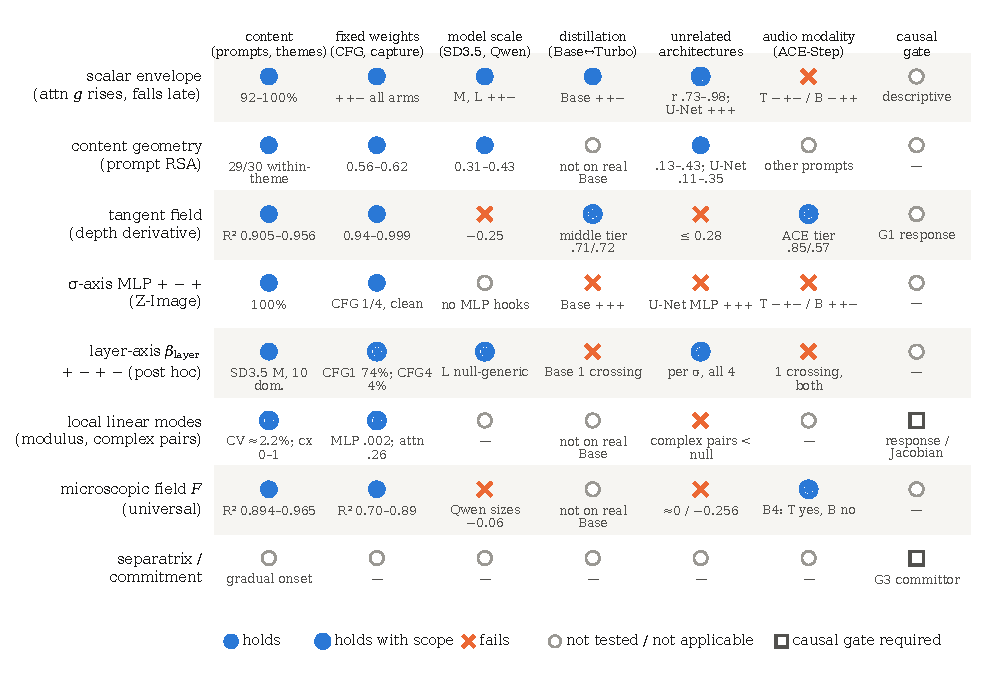
\includegraphics[width=\linewidth,height=0.45\textheight,keepaspectratio]{II-F12_claim_boundary}
 \caption{\textbf{Universality and falsification hierarchy: the claim boundary.} Each row is a candidate structure. Each column asks whether it survives a change of content, fixed weights (guidance, capture), model scale, distillation, unrelated architecture or data modality, and whether a causal gate is still open. The cell text gives the governing number. The distillation column uses the real Z-Image Base (Rounds 11--13) and ACE-Step Base (Round 14); comparisons against \TT{} are same-weights comparisons and sit in the fixed-weights column. What survives is a hierarchy: the coarse scalar envelope recurs everywhere but cannot identify lineage; prompt-content geometry is shared across unrelated models and strongest for the same weights; the tangent field is preserved under fixed weights, held at a middle tier under distillation (0.71/0.72 Z-Image, 0.85/0.57 ACE-Step) and lost across architectures. The $\sigma$-axis $+-+$ is scoped to Z-Image Turbo MLP (real Base: $+++$). Unrelated-architecture cells also give the SD1.5 U-Net of Mode-I where it was measured (post hoc): its prompt geometry is shared with the transformers, while its attention envelope and its MLP envelope both rise over the whole schedule ($+++$). The audio column is ACE-Step of Mode-I, turbo (T) and Base (B): the envelopes follow $-+-$ (T) and $-++$/$++-$ (B), and the layer axis has one crossing in both (preregistered B6 and R12-7); the lineage tangent tier recurs inside audio; prompt geometry and local modes were not compared, because its prompts differ. The layer-axis $+-+-$ (post hoc) holds only with its bootstrap rate and surrogate class, SD3.5 L is null-generic, and the real Z-Image Base conditional branch does not show it. Local linear modes: complex eigenpairs are rarer in the data than under a layer-permutation null, and the modulus tracks profile smoothness (post hoc, Mode-I RC23D), so the rotational reading is retired. A universal microscopic $F$ fails across architectures and across Qwen sizes. Separatrix or commitment statements need the committor gate G3. Not claimed anywhere: RG fixed points or universality classes, thermodynamic criticality, full-state conjugacy (register T5--T6). Per-cell evidence and sources are in \texttt{data/II-F12\_claim\_boundary.csv}. Statuses follow \texttt{R6C\_RELEASE\_CLAIM\_REGISTER.md} and \texttt{R6C\_GATES.md} (v0.19), updated through Round 14.}
 \label{fig:universality}
\end{figure}

%=====================================================================
\section{Open causal mathematics}\label{sec:open}
\begin{itemize}
 \item \textbf{Committor and clones.} A fate boundary is a statement about $q(x)=\Pr(\text{outcome}\mid x)$ \citep{e2010transitionpath}. Measuring it requires cloned continuations from fixed intermediate states and a scored outcome. Transition-path sampling estimates $q$ by shooting continuations \citep{e2006towards,bolhuis2002transition}. Recent work identifies semantic commitment regimes in diffusion models with class-conditional entropy \citep{handke2026entropic} and with symmetry breaking \citep{raya2023spontaneous,biroli2024dynamical,sclocchi2025phase}; our passive telemetry measures neither.
 \item \textbf{Response and Jacobians.} The local maps of \S\ref{sec:linear} are descriptive. A response or susceptibility statement needs paired finite perturbations of the noise or the activations. The level above the tangent of Definition~\ref{def:levels} would be the singular-value growth rates of the depth Jacobian product $J_{\ell_2}\cdots J_{\ell_1}$ over a depth interval, a finite-depth amplification spectrum. Unlike the triple, such rates are invariant under smooth reparametrisation of the hidden state. They are not Lyapunov exponents, because a finite non-autonomous composition of layers has no invariant measure and no long-time limit; where a genuine recurrent state exists, as in a random recurrent network, the full Lyapunov spectrum is now computable \citep{clark2026lyapunov}. Whether a distilled model and its source share such a spectrum, and whether it separates the three tiers of \S\ref{sec:tangent} more sharply than the tangent does, is the natural next test of what a lineage shares, and it needs Jacobian-vector products, which no telemetry in the archive provides.
 \item \textbf{What would change our reading.} Three results would change it. The first has now happened in MLP: a depth-matched unrelated image pair (PixArt-$\Sigma$$\leftrightarrow$Cosmos, Mode-I Round 17) reaches $0.69$ ($0.57$ on the native grid), in the lineage range, so the MLP middle tier is non-specific, while in attention the same pair stays at $0.30$ ($0.20$ native, inside its null). The other two are a capture of the text encoder's own activations that reproduces the Z-Image tier with the denoiser fixed, which would make it an encoder effect (the caption-row values, $0.70$ against $0.71$--$0.72$ on all rows on the 24-point grid, already bound it from above in Z-Image; Mode-I \S5.3); and Jacobian-product spectra that tier differently from the tangent, which would make the tangent a property of the coordinates rather than of the dynamics.
 \item \textbf{Questions that need new captures.} Following the reviews, these are Mode-III tests rather than claims here: more depth-matched unrelated pairs (Round 17 added one), an MLP statistic not dominated by the last block, and a depth-invariant tangent; tiers on text-encoder activations; the identity gate on an SFT checkpoint and swapped files; the actual Z-Image teacher and a Base/Turbo pair at matched guidance; row-split and centred captures of Mochi and SD3.5 Large; a held-out prompt set; a full-resolution activation baseline; and captures that store leading singular values per (layer, step), so that the archive is no longer lossy for these questions.
 \item \textbf{Context-invariant autoregressive observables.} The archive's language-model statistics are running statistics over a growing context, so a per-token phase claim is not available. This is an instrument property: a nested i.i.d.\ sample with no model reproduces the perfect rank correlation with context length for $g$, $gD/n$ and $H$ (Round 9 R9-B1). At matched context the static comparisons remain valid: Qwen2.5 1.5B$\leftrightarrow$3B depth-derivative agreement is $0.63$ ($0.61$--$0.65$, above its layer-permutation null), the pairs with 7B are near zero, and Mistral abliteration keeps the prefill tangent ($0.9998$). Language models with per-token, context-invariant capture and the text-encoder side of text-to-image models are the subject of a separate paper (Mode-III).
 \item \textbf{Massive activations and caption rows.} Uncentred spectra can be dominated by a few extreme channels \citep{sun2024massive,sun2026anatomy}, which in DiTs are modulated by the timestep embedding \citep{gan2025massive} and carry prompt information \citep{turri2026few}. Round 11 ran this test. The Z-Image lineage tangent stays far above unrelated pairs with the eight largest channels removed ($0.68$/$0.43$) and centred ($0.76$/$0.61$), while the SD3.5 Medium depth sequence survives channel removal and vanishes under centring. The larger effect in Z-Image is not a few channels but the caption rows of the joint sequence, which carry at least $98\%$ of the uncentred MLP energy in every layer from 10 to 26 (Fig.~\ref{fig:controls}c); image-row statistics should be the default for joint-sequence models.
 \item \textbf{Origin of the coarse invariants.} The theorems above are agnostic about where the recurring envelope and sign sequences come from. Shared data statistics, the coarse-to-fine ordering imposed by the noise schedule \citep{falck2025fourier}, the residual architecture, or a more general law are all consistent with the archive. A discriminating test holds architecture and objective fixed while changing the spectrum or physics of the training data, and repeats the measurement in a different modality with context-invariant statistics. The U-Net check in Mode-I changes only the block architecture. The audio check changes the modality and loses the depth sign sequence while keeping the plateau; its undistilled checkpoint (Round 14) loses it too, so distillation is not the cause, and the real Z-Image Base loses it as well, so the cause is not the modality either. What the two audio checkpoints do not share (non-autonomy of attention, a susceptibility-like peak, an early prompt-share rise) shows that several properties are checkpoint-specific.
 \item \textbf{Submodule coverage.} The $\tau$-axis $+,-,+$ result needs MLP hooks on Mochi and SD3.5 before it can be called cross-architectural. The other MLPs measured, in the real Z-Image Base, the SD1.5 U-Net and both ACE-Step checkpoints, do not show it.
\end{itemize}

\section*{Data availability}
The raw telemetry and derived cubes are listed, with SHA-256 values, in \texttt{DATA.md} of the Mode-I repository, and will be deposited as a Hugging Face dataset with a DOI; the link and DOI will be added there on deposit. The theorems of this paper do not depend on the data. The project's findings ledger and its internal planning notes are not part of the release; they are available from the author on request for review. The empirical values quoted from Mode-I were checked against its released derived tables, and \texttt{check\_numbers.py} verifies them: the tier, row-set, grid, identity-gate and transfer tables (Mode-I \url{review/r15_deep_dive/review_checks/out/}, RC15--RC32), the Round 5 pooling outputs (\texttt{review/round5/out/}) and the Round 6 S1--S5 outputs (\texttt{review/round6/out/}).

\section*{Code and data}
Scripts for every figure and number are at \url{https://github.com/Z-L-D/mode-II}. Figures are generated by the Python scripts in \texttt{scripts/} (\texttt{make\_all\_figures.py}), which write the plotted values to \texttt{data/}; the review rounds that produced each number, including Rounds 11--14, are in \texttt{review/}, and \texttt{NUMBERS.md} maps every number in this paper to the script and output it comes from. The raw captures of Rounds 11--14 and the derived cubes are listed in \texttt{DATA.md}.

\bibliographystyle{plainnat}
\bibliography{references}

\appendix
\section{Results imported from Mode-I}\label{app:imports}
Every empirical value in this paper comes from Mode-I. The table lists the ones the arguments here lean on, with the evidence class Mode-I gives them (OOS out of sample; LA preregistered with lookahead; PA preregistered on explored archive data; PH post hoc; R review reproduction).
\begin{table}[htbp]
\centering\small
\caption{Mode-I results used in this paper. Values here are rounded to two decimals where Mode-I gives three (for example ACE-Step at 8 steps, $0.80$/$0.59$ here and $0.795$/$0.594$ in Mode-I Table~5).}
\label{tab:imports}
\begin{tabularx}{\linewidth}{@{}>{\raggedright\arraybackslash}p{4.4cm}>{\raggedright\arraybackslash}p{1.9cm}L@{}}
\toprule
Result (Mode-I) & Class & Used here in\\
\midrule
Pooling increments $+0.040$/$+0.050$/$+0.088$ (Round 5) & PA; conditional on equal branch energies & \S3, Table~\ref{tab:poolsize}\\
Related above unrelated, attention tangent, depth-matched & LA (Z-Image), OOS (ACE-Step, Rounds 17--18) & \S\ref{sec:tangent}, \S\ref{sec:universality}\\
Three tiers within related pairs & hypothesis & \S\ref{sec:tangent}\\
FPR bound, depth bands, 12-point reconstruction (RC53, 54, 56) & PH & \S\ref{sec:hierarchy}, \S\ref{sec:tangent}\\
Documented distillation (SD3.5 L$\leftrightarrow$L Turbo) in the middle tier, $0.818$ (24 points), $0.904$ (native) & OOS (24 points), PH (native) & \S\ref{sec:tangent}\\
Branch-energy ratio $\tr M_{\rm cond}/\tr M_{\rm uncond}$, median $1.004$--$1.021$ (Round 18 addendum A) & OOS, descriptive & \S3\\
Activation CKA does not reproduce the tangent's separation (Round 18 addendum B) & OOS & \S\ref{sec:tangent}\\
Tangent not calibrated across depth (RC5) & PH & \S\ref{sec:tangent}, condition (viii)\\
Grid dependence of the tangent (RC1, RC26, RC30); native grid leads (RC33) & PH & \S\ref{sec:tangent}\\
Z-Image Base and Turbo as a sibling pair ($0.55$/$0.77$ native) & LA (24 points), PH (native) & \S\ref{sec:tangent}\\
Residual-field transfer, depth-matched (RC24, RC28) & PH & Finding~\ref{fd:nofield}\\
Shared prompt-relational geometry & PA & \S\ref{sec:content}\\
Near-collinearity of $\log g$ and $H$ (Round 10, RC31) & descriptive & Remark~\ref{rem:dims}\\
Layer-axis sign sequence and its surrogate classes & PA, descriptive & \S\ref{sec:nulls}\\
Relative onset replacing $\sigma_{50}$ & PA & \S\ref{sec:estimators}\\
Caption-row share of Z-Image MLP energy (Round 11) & OOS & condition (vii)\\
\bottomrule
\end{tabularx}
\end{table}

%=====================================================================
\section{Estimator definitions}\label{app:estimators}
\paragraph{Depth profile.} For model $m$ at state $t$, average $z$ over generations, take $(\log g,\log\gap,H)$, $z$-score each across layers, and interpolate onto 24 equally spaced values of $u\in[0,1]$.
\paragraph{Shape.} Pearson correlation of the flattened $24\times3$ profiles at matched $\sigma$, averaged over states.
\paragraph{Tangent.} Cosine of the first differences of the two profiles along $u$, at the nearest $\sigma$ of the second model to each $\sigma$ of the first, averaged over the first model's states.
\paragraph{Plateau onset.} Population state speed $\|\Delta\bar z\|/|\Delta\sigma|$ on $(\log g,\log\gap,H)$; the plateau speed is its median over $\sigma<0.6$; the onset is the first $\sigma$ at which speed falls below twice the plateau.
\paragraph{Seed predictability.} Residuals: $(\log g,\log\gap,H)$ standardised across generations at each step, prompt-mean removed. Ridge ($\alpha=100$) with 5-fold prompt-grouped cross-validation; optional in-fold seed centring.
\paragraph{VR.} Overlapping-difference estimator of \S\ref{sec:estimators} on residual paths after dropping the first state, for $q\in\{2,4,8\}$, without bias correction; reference values from simulated walks, AR(0.8) and i.i.d.\ paths of each channel's own shape, passed through the same estimator.

\paragraph{Residual-field transfer (D15, RC24, RC28).} State per generation, layer and sampling state: $z=(\log g,\log\gap,H)$, standardised per model over all cells. Depth step $\Delta z=z(\ell+1)-z(\ell)$; scaffold $F^{(0)}(u,\tau)$, the population mean of $\Delta z$ at each (layer, state); residual $R=\Delta z-F^{(0)}$, the target. Features: $z-\bar z(\ell,\tau)$, normalised depth $u$ and normalised clock $\tau=\sigma/\sigma_{\max}$ ($\sigma/(1+\sigma)$ first for VP and EDM clocks). Learner: scikit-learn \texttt{HistGradientBoostingRegressor}, 200 iterations, default depth and learning rate, \texttt{random\_state} 0, one regressor per coordinate. Self $R^2$: 5-fold cross-validation grouped by prompt on the target. Cross $R^2$: fitted on all of the source, applied to the target with the target's own scaffold subtracted. $R^2$ pools the three coordinates (one minus total residual over total variance). Shortfall: self minus cross. The archive script for D15 is not in the repository; RC24 re-implements its design as stated here for depth-matched pairs, and RC28 adds the null of Finding~\ref{fd:nofield}.

\section{Surrogate algorithms}\label{app:surrogates}
\paragraph{Surrogate A (layer marginals).} For each layer $\ell$, permute the values $\{g_{p,s}(\ell,\tau)\}$ jointly over all generations and steps. Recompute $\beta$ and the binned conditional mean with the analyzer's own function. 30 draws, seeds $10$--$39$.
\paragraph{Surrogate B (mean field).} For each cell $(\ell,\tau)$, permute $g$ across generations. 30 draws, seeds $500$--$529$. Both surrogates were rerun with 1000 draws each (seeds $10$--$1009$ and $50000$--$50999$; Mode-I review check RC14) and give the same surrogate class in every channel.
\paragraph{Circular-shift backbone null.} For each sampling state independently, circularly shift the standardised depth profile by a random offset along depth; recompute PC1 and entropy effective rank. 999 campaigns.
\paragraph{Straight-line synchronisation surrogate.} Replace each layer's trajectory of each coordinate by its least-squares straight line in step index and recompute the synchronisation index $R(\tau)$ on the population-mean field.
\paragraph{Monotone-warp null.} Re-time each layer's trajectory independently: draw a random monotone map $c:[0,1]\to[0,1]$ with $c(0)=0$, $c(1)=1$ and increments from a Dirichlet(1) distribution, and evaluate the layer's trajectory at $c(u_t)$ by linear interpolation. This keeps every layer's path and its monotonicity and destroys only the cross-layer timing. 500 draws per channel; $p=(1+\#\{R^{\mathrm{null}}_{\max}\ge R_{\max}\})/501$.
\paragraph{Layer-permutation null for tangents.} Permute depth order in one model of the pair and recompute $\rho_{\mathrm{tan}}$; the unrelated pairs' observed values lie at the 39th to 92nd percentile of this null.

\section{Preregistration and falsification record}\label{app:prereg}
\begin{center}\small
\begin{tabularx}{\linewidth}{@{}llcL@{}}
\toprule
Round & SHA-256 prefix, frozen (UTC) & Rows & Confirmed / partial / refuted\\
\midrule
2 & \texttt{2343fd02}, 2026-10-05 11:05 & 28 & 18 / 3 / 7\\
3 & \texttt{d29fdfa6}, 2026-10-05 15:21 & 32 & 1 / -- / 2 (29 not scorable)\\
4 & \texttt{82ef210a}, 2026-10-06 23:01 & 28 & 16 / -- / 6 (5 not scorable; 1 report-only)\\
5 & \texttt{78b250a2}, 2026-10-08 05:24 & 22 & 13 / -- / 9\\
6 & \texttt{c0279f03}, 2026-10-08 07:06 & 22 & 17 / -- / 5\\
7 & \texttt{9012d20f}, 2026-10-08 09:02 & 8 & release audit; consistency checks\\
R3 C (U-Net) & \texttt{efa613eb}, 2026-10-08 15:27 & 3 & 1 / 1 / 1\\
R3 B (ACE-Step) & \texttt{efa613eb}, 2026-10-08 15:27 & 10 & 4 / -- / 4 (B1 gate; B7 not run)\\
8 (correlations) & \texttt{acc578ac}, 2026-10-09 08:30 & 16 & 7 / -- / 9\\
9 (salvage) & \texttt{09c1f170}, 2026-10-09 09:07 & 12 & 6 / -- / 6\\
10 (final sweep) & \texttt{2338e502}, 2026-10-09 22:27 & 2 & 0 / -- / 2\\
11 (uncentred controls) & \texttt{3834abb0}, 2026-10-17 13:22 & 7 & 2 / -- / 5\\
12 (real Base, lineage) & \texttt{ad06a1bb}, 2026-10-18 06:21 & 9 & 6 / -- / 0 (gate, rule, descriptive)\\
13 (split-half holdout) & \texttt{47cf1e67}, 2026-10-27 22:14 & 6 & 6 / -- / 0\\
14 (ACE-Step Base) & \texttt{dc997f6d}, 2026-11-05 18:56 & 6 + 10 & 4 / -- / 2; B replay 3 / -- / 5\\
15 (held-out replications) & \texttt{3acbb027}, 2026-11-05 21:23 & 7 & 6 / -- / 1\\
16 (ACE-Step turbo, 8 steps) & \texttt{a3b59c92}, 2026-11-06 15:05 & 9 & 5 / -- / 3 (gate)\\
17 (tier controls) & \texttt{16ccbe54}, 2026-11-07 22:07 & 5 & 2 / -- / 1 (gate, rule)\\
18 (documented distillation, session, shift) & \texttt{6db32be7}, 2026-11-09 10:32 & 7 & 6 / -- / 0 (gate)\\
18 addendum B (activation CKA) & \texttt{24a739d4}, 2026-11-09 12:42 & 4 & 1 / -- / 1 (rules)\\
\bottomrule
\end{tabularx}
\end{center}
Of the 253 rows, 197 were scored, 8 are consistency checks (Round 7), 34 were not scorable as captured (29 in Round 3, 5 in Round 4), and 14 are gates, rule outputs, descriptive or report-only rows, or predictions not run. Claims removed by refutations or audits and therefore absent from this paper: a mid-run synchronisation pulse as a phase event; a universal semantic commitment time; universal seed collapse; a universal passive susceptibility peak; a universal crossing-ratio ladder (``ratio 2''); a compressed learned clock between 25- and 8-step Turbo (replaced by equal-$\sigma$ registration); kinematic $\varphi$ closure; an autoregressive multiscale $\beta$ anomaly; an architecture ordering of scalar envelopes; and a universal damped-oscillator local mode. Also not supported: a lineage reading of the archive campaign labelled ``Z-Image Base'' (it is \TT{}; lineage rests on real Base captures, \S\ref{sec:tangent}); the image/video specificity of the depth sign sequence; and the clock-axis contraction as a Z-Image property (it is a Turbo caption-row property). Rounds 11--18 are scored in Mode-I: R11-1 and R11-2 (thresholds anchored on the \TT{}$\leftrightarrow$ZIT pair), R11-5, R11-6 and R11-7, R14-2 and R14-6, R16-1, R16-4 and R16-8, and R17-1 (the MLP bottom tier) are refuted; the Round 12 lineage tests, R12-6 and R16-2 hold, and R17-2 places SD3 Medium$\leftrightarrow$SD3.5 Medium in the middle tier; R18-1, R18-2 and R18-4 hold (SD3.5 Large$\leftrightarrow$Large Turbo in the middle tier, SD3.5 Large across sessions, the sibling value at Base's shift 6), R18-3a and R18-3b pass by their rules as an exact replay, and of addendum B, B1 holds, B2 and B3 are not supported and B4 is refuted.


\clearpage
\setcounter{section}{0}\setcounter{table}{0}\setcounter{figure}{0}
\renewcommand{\thesection}{S\arabic{section}}\renewcommand{\thetable}{S\arabic{table}}\renewcommand{\thefigure}{S\arabic{figure}}
\renewcommand{\theHsection}{S\arabic{section}}\renewcommand{\theHtable}{S\arabic{table}}\renewcommand{\theHfigure}{S\arabic{figure}}
\begin{center}{\Large\bfseries Supplementary material}\\[4pt]\small Mode-II: Projection, Pooling and Tangent Agreement. Sections, tables and figures here are numbered S1, S2, \ldots; the main text points to each.\end{center}
\addcontentsline{toc}{section}{Supplementary material}
% Supplementary material for Mode-II, input at the end of main.tex
\section{Closure ladder}\label{supp:closure}
The held-out $R^2$ values behind \S\ref{sec:flow}, transcribed from the findings ledger.

\begin{figure}[h]
 \centering
 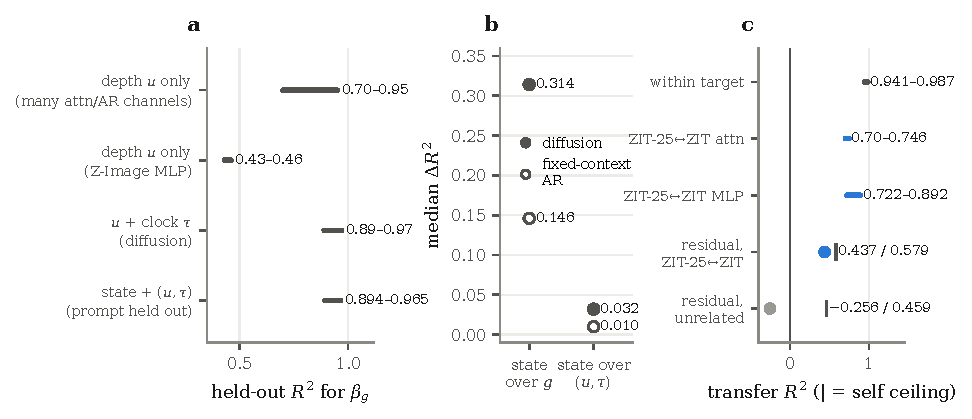
\includegraphics[width=\linewidth]{II-F4_closure_ladder}
 \caption{\textbf{Nonautonomous closure ladder.} Values are transcribed from the findings ledger. The ledger reports ranges and medians, not per-channel tables, so ranges are drawn as intervals. (a) Held-out $R^2$ for the layer-direction flow $\beta_g$: depth $u$ alone: 0.70--0.95 in many attention/AR channels, but only 0.43--0.46 in Z-Image MLP; $u$ plus the clock $\tau$: 0.89--0.97 in diffusion; local state plus coordinates with whole prompts held out: 0.894--0.965 (D01). (b) Median incremental $R^2$. The spectral state $[g,{\rm gap},H]$ adds $+0.314$ (diffusion) and $+0.146$ (fixed-context AR) over $g$ alone. Once a flexible learner has $(u,\tau)$, the full state adds only $+0.032$ (diffusion) and $+0.010$ (AR), or $+0.014$ overall. Under the frozen minimal-sufficiency rule, 7/12 channels need only $(u,\tau)$ and 5/12 need $g+u+\tau$ (D08/D09). This ladder is close to true by construction once the scaffold holds $96\%$ of the variance (\S\ref{sec:flow}); it describes how the measured manifold is parametrised, and the non-autonomy argument rests on the transfer results in (c) and Table~\ref{tab:transfer}. (c) Vector-field transfer: within target: 0.941--0.987; \TT{}$\leftrightarrow$ZIT (same Turbo weights): attention 0.700--0.746, MLP 0.722--0.892 (D03); residual after scaffold subtraction: \TT{}$\leftrightarrow$ZIT 0.437 against a self ceiling of 0.579, unrelated pairs $-0.256$ against $\approx0.459$ (D15). Transfer into Mochi and SD3.5 M/L is "approximately zero or negative" (D03). No value is tabulated for it, so it is not plotted. Together these support a model-specific nonautonomous family $\dot z=F_m^{(0)}(u,\tau)+R_m(z,u,\tau)$ and reject a universal autonomous $\beta(g)$ or a universal microscopic $F$ (register T5). Sources: ledger cards "Depth coordinate is a major explanatory variable" (script 15), "Cross-substrate CoS state\ldots{}" (script 11), D01, D03, D08/D09 and D15.}
 \label{fig:closure}
\end{figure}

\section{Intrinsic arc-length reparameterisation}\label{app:arclength}
Reparameterising each coarse curve by cumulative spectral arc length raises unrelated and cross-channel correlations by $+0.057$ on average, changes the comparison of \TT{} with ZIT (the same Turbo weights) by $-0.004$, and the preregistered paired test is not significant ($p\approx0.105$, D17). Arc length is therefore not a decisive universal progress variable.

\section{Legacy rebound and complex-mode study}\label{app:legacy}
Fitting $z(\ell+1)=Az(\ell)+b$ with $z=(g,-\gap,H)$ on the final rebound branch of SD3.5 Medium depth profiles gives a complex-conjugate pair with modulus below one at all three resolutions, retained in 500 of 500 generation-cluster bootstraps, median moduli $0.526$ ($512$), $0.501$ ($768$), $0.400$ ($1024$). These files were recorded with a hook that substitutes an exponential-moving-average attention path whenever it is registered, on a single prompt; in a matched CFG study the complex mode exists only in steps 0--9, and over all 100 steps CFG 1.0 has no complex pair. We report the study as a historical exploration with that instrument caveat, not as release evidence.

\section{Envelope trend ratios and coordinate collinearity}\label{supp:kappa}
\begin{table}[htbp]
\centering\small
\caption{Trend-dominance floor of Proposition~7 per pair (post hoc, Mode-I RC25). Layer-mean attention $g$ of the five archive campaigns on a common $\sigma$ grid; trend $T$ = the five-model mean envelope (descriptive: it contains both models of each pair). $\kappa=\operatorname{Var}(r)/(\alpha^2\operatorname{Var}T)$; floor $=(1-\sqrt{\kappa_a\kappa_b})/\sqrt{(1+\kappa_a)(1+\kappa_b)}$; observed: the envelope correlation. Values for $T$ linear in $\sigma$ are in \texttt{rc25\_kappa\_pairs.csv}.}
\label{tab:kappa}
\begin{tabular}{llcccc}
\toprule
Pair & Relation & $\kappa_a$ & $\kappa_b$ & Floor & Observed\\
\midrule
ZIT $\leftrightarrow$ Mochi & unrelated & 0.078 & 0.355 & 0.690 & 0.707\\
ZIT $\leftrightarrow$ SD3.5 M & unrelated & 0.078 & 0.156 & 0.797 & 0.969\\
ZIT $\leftrightarrow$ SD3.5 L & unrelated & 0.078 & 0.010 & 0.931 & 0.976\\
\TT{} $\leftrightarrow$ Mochi & unrelated & 0.042 & 0.355 & 0.739 & 0.923\\
\TT{} $\leftrightarrow$ SD3.5 M & unrelated & 0.042 & 0.156 & 0.837 & 0.846\\
\TT{} $\leftrightarrow$ SD3.5 L & unrelated & 0.042 & 0.010 & 0.954 & 0.960\\
Mochi $\leftrightarrow$ SD3.5 M & unrelated & 0.355 & 0.156 & 0.611 & 0.624\\
Mochi $\leftrightarrow$ SD3.5 L & unrelated & 0.355 & 0.010 & 0.803 & 0.808\\
SD3.5 M $\leftrightarrow$ SD3.5 L & same family & 0.156 & 0.010 & 0.888 & 0.958\\
\bottomrule
\end{tabular}
\end{table}

\begin{table}[htbp]
\centering\small
\caption{Spearman correlations between the coordinates over all (generation, state, layer) cells of each cube (post hoc, Mode-I RC31). The first seven rows are the archive cubes behind Remark~\ref{rem:dims} (its range, $0.93$--$0.97$ and $-0.79$ to $-0.20$); the rest are the Round 12--17 cubes.}
\label{tab:collin}
\begin{tabular}{llrccc}
\toprule
Cube & Hook & Cells & $\log g$, $H$ & $\log g$, $\log\gap$ & $H$, $\log\gap$\\
\midrule
ZIT & attn & 115{,}200 & 0.963 & $-$0.730 & $-$0.660\\
ZIT & MLP & 115{,}200 & 0.969 & $-$0.456 & $-$0.304\\
\TT{} & attn & 357{,}000 & 0.969 & $-$0.760 & $-$0.709\\
\TT{} & MLP & 357{,}000 & 0.972 & $-$0.513 & $-$0.384\\
Mochi & attn & 688{,}320 & 0.974 & $-$0.787 & $-$0.745\\
SD3.5 M & attn & 460{,}800 & 0.939 & $-$0.203 & $-$0.059\\
SD3.5 L & attn & 516{,}040 & 0.926 & $-$0.516 & $-$0.364\\
Z1 (Base) & attn & 359{,}250 & 0.969 & $-$0.780 & $-$0.724\\
Z1 (Base) & MLP & 358{,}500 & 0.952 & $-$0.527 & $-$0.333\\
Z3 (Turbo{,} Base settings) & attn & 90{,}000 & 0.956 & $-$0.698 & $-$0.612\\
Z3 (Turbo{,} Base settings) & MLP & 90{,}000 & 0.972 & $-$0.505 & $-$0.363\\
ACE-Step Base & attn & 72{,}000 & 0.962 & $-$0.297 & $-$0.250\\
ACE-Step Base & MLP & 72{,}000 & 0.960 & $-$0.337 & $-$0.382\\
ACE-Step turbo & attn & 17{,}280 & 0.955 & $-$0.134 & $-$0.060\\
ACE-Step turbo & MLP & 17{,}280 & 0.976 & 0.087 & 0.096\\
SD3 M & attn & 40{,}320 & 0.914 & $-$0.433 & $-$0.249\\
PixArt-$\Sigma$ & attn & 33{,}600 & 0.967 & $-$0.476 & $-$0.341\\
PixArt-$\Sigma$ & MLP & 33{,}600 & 0.962 & $-$0.389 & $-$0.184\\
Cosmos-Predict2 2B & attn & 58{,}800 & 0.851 & $-$0.280 & $-$0.059\\
Cosmos-Predict2 2B & MLP & 58{,}800 & 0.862 & $-$0.487 & $-$0.133\\
\bottomrule
\end{tabular}
\end{table}

\section{Supplementary figures}\label{app:supp}

\begin{figure}[p]
 \centering
 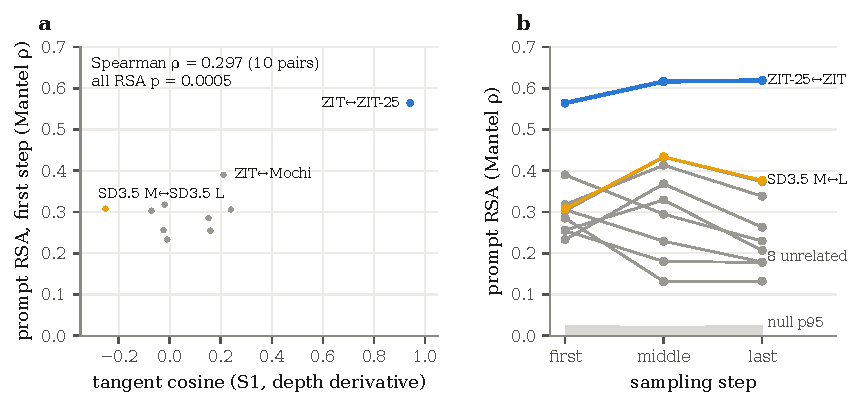
\includegraphics[width=\linewidth]{II-F7_content_vs_dynamics}
 \caption{\textbf{Content geometry and dynamics are different quotients.} (a) For each of the 10 model pairs, the first-step prompt RSA is plotted against the tangent cosine. The RSA is a Mantel $\rho$ between $117\times117$ prompt-distance matrices, with $p=0.0005$ for every pair against its own prompt-permutation null. The rank coupling is weak (Spearman $\rho=0.297$, preregistered S2g). (b) RSA at the first, middle and last step. Unrelated pairs score 0.13--0.43 and \TT{}$\leftrightarrow$ZIT (same weights) 0.56--0.62. Every value lies far above its permutation-null p95 ($\approx0.02$, shaded). Shared content organization exists across unrelated architectures, beyond themes and prompt text (P2), and without a shared microscopic flow. The two are distinct equivalence relations. Sources: \texttt{review/round6/out/S2\_rsa.csv}, \texttt{S1\_hierarchy.csv}; register \#19, T3.}
 \label{fig:content}
\end{figure}

\begin{figure}[p]
 \centering
 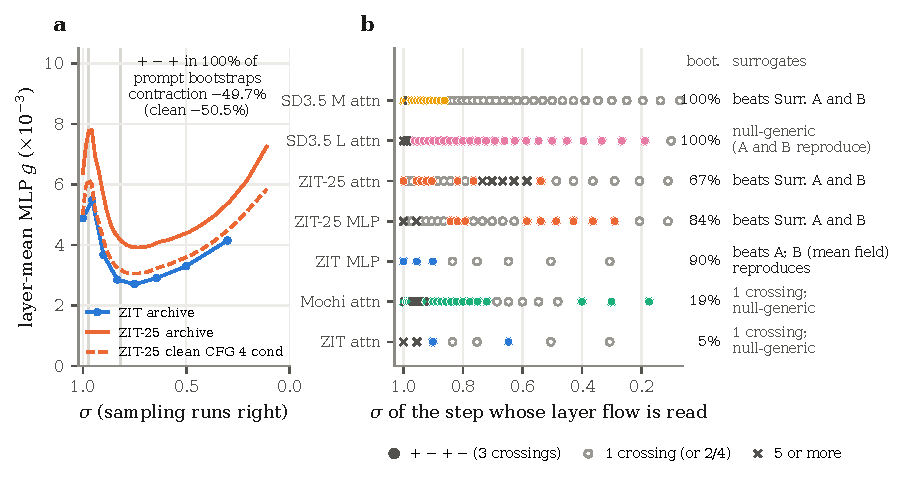
\includegraphics[width=\linewidth]{II-F8_two_axis_topology}
 \caption{\textbf{Two different phase constructions; do not conflate them.} (a) Sampling-clock axis, Z-Image MLP only. Population-mean, layer-mean MLP $g(\sigma)$ is shown for ZIT (8 steps), \TT{} (archive, pooled CFG 4) and the clean \TT{} CFG 4 cond branch, recomputed from the raw cubes. All three are Z-Image Turbo (the 25-step archive files are labelled ZIB); the real Base MLP gives $+++$ (Round 11, not drawn). The three-segment fit gives $+-+$ in 100\% of 1000 prompt bootstraps in every arm (S4a--b). The contraction is $-49.7\%$ in the archive and $-50.5\%$ on the clean branch. Vertical lines mark the \TT{} archive breakpoints, $\sigma=0.972$ and $0.818$. Attention follows a different curve ($++-$) in all five archive channels (S4e, P1), so the $\sigma$-axis result is scoped to Z-Image Turbo MLP. (b) Layer axis, post hoc (analyzer replay A2--A4). The sign pattern of $\beta_{\rm layer}(g)$, binned against $g$, is shown at each sampling step. Right-hand columns give the whole-run generation-bootstrap rate of $+-+-$ and the surrogate class: SD3.5 M attention: 100\%, beats Surrogates A and B; SD3.5 L attention: 100\%, \textbf{null-generic} (per-layer marginals alone reproduce it); \TT{} attention: 67\%, beats A and B; \TT{} MLP: 84\%, beats A and B; ZIT MLP: 90\%, beats A, but B (the mean field $g(L,\sigma)$) reproduces it; Mochi and ZIT attention: a single, null-generic crossing. Not drawn: the real Z-Image Base conditional branch and both ACE-Step checkpoints give one crossing (Rounds 12 and 14; Mode-I Fig.~14). Report the layer-axis pattern per $\sigma$ or with its bootstrap rate and surrogate class, never as one crossing count. Neither panel defines a phase boundary or a separatrix. Sources: \texttt{review/round6/out/S4\_topology.csv}, \texttt{A2\_beta\_layer\_bootstrap.csv}, \texttt{A4\_beta\_layer\_per\_step.csv}, \texttt{A4\_beta\_layer\_surrogates.csv}; raw cubes for the curves in (a); register \#1.}
 \label{fig:topology}
\end{figure}

\begin{figure}[h]
 \centering
 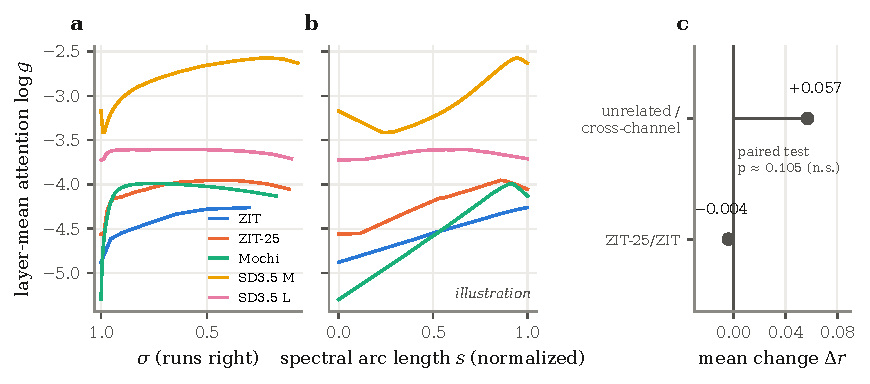
\includegraphics[width=\linewidth]{II-S1_intrinsic_progress}
 \caption{\textbf{Intrinsic progress gives no decisive universal quotient (negative result).} (a,b) Illustration on data: layer-mean attention $\log g$ for the five archive models, plotted against $\sigma$ (a) and against normalized cumulative spectral arc length (b). Here arc length is re-implemented as the path length of the z-scored layer-mean $(\log g,\log{\rm gap},H)$. It shows the reparameterization only and is not the D17 computation. (c) Ledger D17: arc-length reparameterization raises unrelated and cross-channel envelope correlation by $+0.057$ on average. The preregistered paired test is not significant ($p\approx0.105$). \TT{}/ZIT (same weights) changes by $-0.004$. A universal intrinsic-progress quotient is therefore not established.}
 \label{fig:S1}
\end{figure}

\begin{figure}[h]
 \centering
 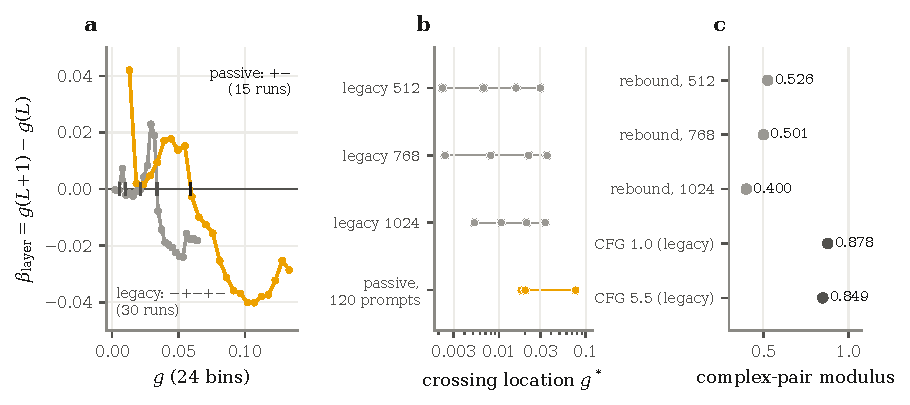
\includegraphics[width=\linewidth]{II-S2_legacy_rebound}
 \caption{\textbf{Legacy rebound and local complex mode: historical, instrument-labelled.} Everything marked \emph{legacy} comes from EMAG-schema files written by an older EMAG-guider build, whose measuring hook substitutes the stale EMA attention. It is shown as the history of the mathematical exploration and is not release evidence. (a) 24-bin $\beta_{\rm layer}(g)$ for a matched 100-step SD3.5 M study with the same prompt and schedule. The 30 legacy-schema runs give $-+-+-$ (four crossings); the 15 current passive runs give $+-$ (one crossing, $g^*=0.059$). Legacy $g$ sits about $10\times$ below passive $g$. The ledger reports the four-crossing pattern for 30/30 single legacy generations and 0/60 single passive prompts. (b) Crossing locations on the legacy resolution suite (512, 768 and 1024 px, single prompt; four crossings each) and on the passive 120-prompt SD3.5 M campaign (three crossings, $g^*=0.018/0.020/0.077$). (c) Complex-pair modulus of the local affine map: on the legacy rebound branch: 0.526, 0.501 and 0.400; in the legacy CFG $1.0\to5.5$ study, steps 0--9: 0.878 [0.862, 0.891] $\to$ 0.849 [0.836, 0.861]. Over all 100 steps of that study, CFG 1.0 has no complex pair. Sources: \texttt{review/round5/reviewer\_v016/results/B7\_MATCHED100\_*}; ledger rebound cards with their v0.12--v0.15 annotations.}
 \label{fig:S2}
\end{figure}


\end{document}
